\documentclass{ieeeaccess}
\usepackage{cite}
\usepackage{amsmath,amssymb,amsfonts}
% \usepackage{algorithmic}
\usepackage{graphicx}
\usepackage{textcomp}

\usepackage{bm}
\makeatletter
\AtBeginDocument{\DeclareMathVersion{bold}
\SetSymbolFont{operators}{bold}{T1}{times}{b}{n}
\SetSymbolFont{NewLetters}{bold}{T1}{times}{b}{it}
\SetMathAlphabet{\mathrm}{bold}{T1}{times}{b}{n}
\SetMathAlphabet{\mathit}{bold}{T1}{times}{b}{it}
\SetMathAlphabet{\mathbf}{bold}{T1}{times}{b}{n}
\SetMathAlphabet{\mathtt}{bold}{OT1}{pcr}{b}{n}
\SetSymbolFont{symbols}{bold}{OMS}{cmsy}{b}{n}
\renewcommand\boldmath{\@nomath\boldmath\mathversion{bold}}}
\makeatother

\def\BibTeX{{\rm B\kern-.05em{\sc i\kern-.025em b}\kern-.08em
    T\kern-.1667em\lower.7ex\hbox{E}\kern-.125emX}}

%Your document starts from here ___________________________________________________
\usepackage{array}
\usepackage[caption=false,font=normalsize,labelfont=sf,textfont=sf]{subfig}
\usepackage{stfloats}
\usepackage{url}
\usepackage{verbatim}
\usepackage{graphicx}
\usepackage{cite}
\usepackage{algorithm}
\usepackage{algpseudocode}
% \usepackage{xcolor} %added for in-line comments %removed for now since it was causing issues with the template
\usepackage[author={TestAuthor}]{pdfcomment} % PDF Comment Package

\usepackage{soul}
\usepackage{xcolor}
\sethlcolor{yellow!50}


\newcommand{\blockcomment}[1]{}

\usepackage{xcolor}
\usepackage{siunitx}
% \newcommand{\highlight}[1]{\colorbox{yellow!50}{#1}}


% \DeclareRobustCommand{\citehighlight}{\hl{\cite}}

% Highlighted version
% \newcommand{\highlight}[1]{\hl{#1}}
% when done can remove highlights with this instead
\newcommand{\highlight}[1]{#1}

\DeclareMathOperator*{\fitness}{fitness}
\DeclareMathOperator*{\random}{random}
\DeclareMathOperator*{\mutate}{mutate}

\begin{document}
\history{Date of publication xxxx 00, 0000, date of current version xxxx 00, 0000.}
\doi{10.1109/ACCESS.2024.0429000}

\title{Bitstream Evolution: an Open-Source FPGA Intrinsic Evolvable Hardware Toolkit}
\author{\uppercase{Allyn Loyd}\authorrefmark{1,2}, 
\uppercase{Daniel Gaull}\authorrefmark{1,3}, 
\uppercase{Logan Manthey}\authorrefmark{1,4},
\uppercase{ Nicklas Carpenter}\authorrefmark{5},
\uppercase{ Derek Whitley}\authorrefmark{1,4},
\IEEEmembership{Member, IEEE}, and
\uppercase{  Jason A. Yoder}
\authorrefmark{1},
\IEEEmembership{Member, IEEE}}

\address[1]{Rose-Hulman Institute of Technology, Terre Haute, IN 47803 USA}
\address[2]{ University of Houston, Houston, TX 77204 USA}
\address[3]{Tesla, Inc. Austin, TX 78725 USA}
\address[4]{Vivum AI, Bloomington, IN, 47401 USA}
\address[5]{University of Arizona, Tucson, Arizona 85721 USA}

% \tfootnote{``This work was supported in part by the U.S. Department of Commerce under Grant BS123456.''}
% \tfootnote{This paragraph of the first footnote will contain support
% information, including sponsor and financial support acknowledgment. For
% example, ``This work was supported in part by the U.S. Department of
% Commerce under Grant BS123456.''}

\markboth
{Loyd \headeretal: Preparation of Papers for IEEE TRANSACTIONS and JOURNALS}
{Loyd \headeretal: Preparation of Papers for IEEE TRANSACTIONS and JOURNALS}

\corresp{Corresponding author: Jason A. Yoder (e-mail: yoder1@rose-hulman.edu).}

%(e-mail: loydma@rose-hulman.edu, gaulldj@rose-hulman.edu, manthelt@rose-hulman.edu, yoder1@rose-hulman.edu)
%Nicklas Carpenter is with University of Arizona (e-mail: npcarpenter@arizona.edu)
%Derek Whitley is CTO and co-founder at Vivum AI and Visiting Assistant Professor at Rose-Hulman Institute of Technology (e-mail: derek@vivum.ai )



\begin{abstract}
% area of interest
The field of intrinsic, bitstream-level, evolvable hardware has recently been resurrected and interest in the area has 
% \pdfmarkupcomment[markup=Squiggly,color=green]
begun to grow. %}{move to the front}.
% goal
This paper presents a low barrier-to-entry software and hardware platform allowing evolvable hardware researchers to conduct experiments, visualize results, and share data. 
% how to accomplish goal
The system's open-source software is designed to enable iterative enhancements so that contributors from around the world can participate. 
% support reaching goal
To encourage community development, we detail the process and results of several of our experiments, which can be used as a reference for further study.
% demonstrative results
Additionally, we discuss the results of our experiments, focusing in particular on their implications with respect to the question of robustness and transferability of evolved hardware circuits. Our results demonstrate significant potential for evolving circuits that not only maintain long-term functionality but can also operate effectively outside their original evolutionary environments. These results demonstrate the feasibility of intrinsic, bitstream level evolution which, in the long run, could increase the efficiency and lower the power requirements of modern computing and artificial intelligence systems.
% future directions
We discuss open questions for the field and directions for future work including stability, transferability, robustness, quality diversity, signal processing, and security.
\end{abstract}

\begin{keywords}
analog computing, bitstream-level evolution, circuit robustness, circuit transferability, evolvable hardware, evolutionary computation, field-programmable gate array evolution, intrinsic evolvable hardware, intrinsic analog evolvable hardware design

%Enter key words or phrases in alphabetical
% order, separated by commas. Autocorrelation, beamforming, communications technology, dictionary learning, feedback, fMRI, mmWave, multipath, system design, multipath, slight fault, underlubrication fault.
\end{keywords}

\titlepgskip=-21pt

\maketitle

\section{Introduction}
\label{sec:introduction}
\IEEEPARstart{E}{volvable} hardware offers an innovative approach to circuit design, challenging traditional human-designed circuits under certain circumstances.
% why is it important?
This field stands to address computing efficiency and power consumption challenges inherent in conventional \textit{digital} hardware, which often rely on standardized abstractions such as clock signals and discrete voltage levels. 
% what is problem?
These abstractions, while easier for humans to comprehend (and granting certain guarantees of reliability), can lead to inefficiencies in power and computation. 
% how to address? analog
\textit{Analog} computing, which does not necessitate clock synchronization and discrete voltage levels, has the power to enhance computing power and reduce energy consumption.
% problem with solution? design
However, designing effective analog circuits is complex, especially given the non-linear characteristics of semiconductors and environmental variations.
% solution to design? EHW
Within the field of evolvable hardware, evolutionary algorithms can be applied to reconfigurable hardware to evolve analog circuits intrinsically. The evaluation of the circuits embedded in the hardware %and local environment
can leverage non-linearities to enhance rather than degrade their performance.
% evidence  of the approach being powerful
This approach, exemplified by Adrian Thompson's work in evolving a tone discriminator with minimal logic gates \cite{Thompson1998OnEvolution}, demonstrates the potential of evolvable hardware to perform complex tasks efficiently.
This result, along with several other experiments, has only recently been reproduced on modern hardware \cite{HoffmannCoBEA:Bitstreams}, after a hiatus due to several factors \cite{Whitley2021ResurrectingHardware}.


% what is the area and how do we approach it
This recently resurrected research area is one subdomain of evolvable hardware, which is itself a broad field, divisible into several categories of practice - intrinsic vs extrinsic, analog vs digital, and adaptive hardware vs evolvable hardware design.
% 3. goal design circuits
As a whole, evolvable hardware aims to offer alternative approaches to the traditional, human-engineered designs of circuits.
% 4. EHD specifically
The toolkit we report in this paper is focused on intrinsic analog evolvable hardware design (EHD).
% Feedback - explain EHD
% Feedback addressed in below sentence in a way that seems to flow better
%EHD is the process of evolving a final circuit design to be used in its target environment.
% 5. EHD - means no online changes
Consistent with the EHD approach, in which one final circuit design is created during the evolutionary phase, we aim to evolve a final circuit that does not require changes during its operation. 
% 6. no online changes means we need transferability and robustness
Due to this constraint, we must consider methods of improving circuits’ transferability and robustness, which we explore in this paper. 
% 7. intrinsic necessary for analog circuits
Given that analog circuits may be influenced by subtle environmental factors --- unlike digital circuits which abstract them away ---
we chose to evolve circuits intrinsically, evaluating fitness from physical circuits, rather than extrinsically --- i.e. via simulation --- to ensure the best performance on actual hardware. 
% 8. challenges and potential, need for this toolkit
%This approach faces substantial challenges, but also presents great opportunities to take advantage of signals and timescales that are below the level of abstraction in conventional digital hardware. 
% Feedback - clarify why this approach can increase efficiency
This approach presents great opportunities to take advantage of signals and timescales that are below the level of abstraction in conventional digital hardware --- allowing for evolution to produce more power-efficient circuits than could be designed by humans.
% With previous point, add in a note about the challenges that this approach faces
However, this avenue also introduces the challenge of evolution relying too heavily on noise that is inconsistent between environments --- resulting in the aforementioned focus on transferability and robustness.

One longstanding challenge for research in this field is the barrier-to-entry as existing efforts tend to require expensive hardware \cite{Garvie2020EvolvedControllers} and complex configuration to begin even basic experimentation. Our key contribution in this paper is lowering the barrier-to-entry substantially through the communication of the \textit{Bitstream Evolution} platform as a well-tested and easy-to-use system. Our publicly-shared code repository can be found at \href{https://github.com/evolvablehardware/BitstreamEvolution}{github.com/evolvablehardware/BitstreamEvolution}. 

The system enables research in this subdomain of evolvable hardware by a wider range of people than ever possible before. There are many interesting research questions in the field and our inexpensive platform allows progress to be made in answering them. Our initial use of this technology platform has allowed us to explore the 
1) robustness of different types of circuits, 
2) methods to bridge the gaps between large timescales (an analog circuit, operating on the order of \textit{nanoseconds} or less, producing an oscillating signal on the order of \textit{kilohertz}), 
3) algorithms to improve the transferability and robustness of circuits, as well as
4) explore what functionality can be evolved on modern hardware.





In the remaining sections of this paper, we will discuss in greater depth the goals (\ref{sec_goals}) for this version of the framework, previous related work (\ref{sec_related_work}), as well as an overview (\ref{sec_framework}) of the \textit{Bitstream Evolution} framework as a whole. 
In addition, we report on preliminary results (\ref{sec_results}) in evolving oscillators, and evaluations of the sensitivity and transferability of evolved circuits. Finally, we present a discussion (\ref{sec_discussion}) the implications of the results as well as future directions (\ref{sec_future_work}) of this research, some of which is under development and ongoing at this time.

%%%%%%%%%%%%%%%%%%%%%%%%%%%%%%%%%%%%%%%%%%%%%%%%%%%%%%%%%%%%%%%%%%%%%%%%%%%%%%%%
%
%                     GOALS II.
%
%%%%%%%%%%%%%%%%%%%%%%%%%%%%%%%%%%%%%%%%%%%%%%%%%%%%%%%%%%%%%%%%%%%%%%%%%%%%%%%%




% what is limited or problematic about our knowledge or work thus far
% what will we do to address these limitations?
\section{Goals}\label{sec_goals}

%%  Need to determine the specific list of goals we have and express them plainly up front and then elaborate
  % 1.  Accessible Platform
  %     a. inexpensive
  %     b. well-tested
  %     c. well-documented
  %     d. designed for verification (new func)

The main goal of this framework is to provide a widely accessible research and development platform. %Because experiments take such a long time to run, 
Greater community involvement has the potential to rapidly increase progress in the field. Our framework, \textit{Bitstream Evolution}, is a well-tested, easy-to-use, and easily configurable software framework for intrinsic analog FPGA evolution. 
Moreover, \textit{Bitstream Evolution} is an open-source platform that utilizes relatively inexpensive and readily available \highlight{third-party} hardware components, making it an affordable option compared to most existing evolvable hardware research configurations (an iCE40 FPGA and Arduino Nano MCU have a combined cost of less than \$200, as of \highlight{June 2025}, via online suppliers such as digikey.com and store.arduino.cc).
In addition to software used to control and measure signals from the FPGA, there are simple simulation modes available to verify the functionality of specific software modules such as fitness functions and evolution algorithms.


  % 2.  Open Science Oriented
  %     a. Open Source
  %     b. Sphinx for easily accessible docs?
  %     c. Public bitstream population repo?

We aim to foster an open science community through several design choices. First, we have chosen to develop our software with an open-source license. Second, we use a \href{https://github.com/evolvablehardware/BitstreamEvolutionPopulations}{publicly-shared repository} of evolved bitstream populations to allow researchers to reuse preexisting evolved populations and contribute new ones. 

%Finally, we have begun integrating an API documentation tool, \href{https://www.sphinx-doc.org/}{Sphinx}, to provide web-accessible documentation.
  

% 3.  Research Agenda - Open Questions
%     A.  Best Practices for EAs with this challenge
%         (selection, population size, elitism, selection, diversity, injected random circuits?, fitness function (tolerant/sensitive))
 

In line with our goals of accessibility and open science, we have identified several open research areas; we report on our preliminary efforts in Section \ref{sec_results}. %Because intrinsic analog EHW has only recently been resurrected, 
A key goal for the new era is exploring intrinsic evolution on modern hardware. We aim to identify best practices for evolutionary algorithms and evaluate the impact of various design decisions on noisy fitness functions \cite{Dang2015EfficientAlgorithms}.

%     B. Properties of evolved Noise
%        (VAR-MAX, sensitivity, reliability, etc)
We also want to answer questions about the characteristics of \textit{generative} circuits which were evolved to utilize noise (they are not provided any explicit input signals). How easily are such circuits evolved? Are such evolved circuits robust in their behavior over time? In the same or different environment?
%In different environments?% How is circuit behavior impacted by environmental factors such as temperature and humidity?

%     C.  Dynamical process at different timescales
%         (nano vs. kilo, 1k, 10k, 100k, etc, evolved RADIO )
Similarly, there are open questions about the relative challenge and reliability of circuits that exhibit dynamics at different timescales. Are circuit behaviors more easily evolved at certain frequencies? %Do oscillatory circuits become more or less reliable at higher frequencies?
What causes any observed differences in behavior? %How can we improve  hardware and algorithm design?

%     D.  Robustness
%         (sensitivity, number of samples/passes, env factors, time factors)
Valuable questions remain about evolving robust circuits. What techniques can adjust algorithms, fitness functions, and hardware to enhance circuit consistency? Does varying the operational envelope during evolution improve self-consistency? Can multiple evaluations of a single circuit within a fitness function improve self-consistency?

%     E.  Transferability
%         (ABABA, ABCABC, A/B/C/D (combined population as seed)   
Beyond robustness, we aim to investigate circuit transferability. Specifically, how do circuits evolved on one FPGA perform on others? We seek methods to improve transferability, such as parallel evaluation on multiple FPGAs or alternating evolution on different FPGAs (see Section \ref{sec_results}). %Additionally, maintaining a diverse collection of circuits may broaden transferability.




In summary, we hope that the use of this highly accessible system will help address questions in areas of 1) best practices for evolutionary algorithms on modern hardware, 2) characterizing properties of circuits evolved for generative tasks utilizing noise,  3) impacts of timescale on the evolution and behavior of circuits, 4) identifying effective methods for increasing robustness and 5) transferability for circuits. %, as well as exploring the development and applications of 6) quality diversity algorithms for evolvable hardware.
We hope to see the growth of a research community with standards of open source, open science, and community collaboration. 

%Beyond these initial areas of immediate opportunity for discovery, we have additional long-term goals, which we discuss in future work (Section \ref{sec_future_work}).

\section{Related Work}\label{sec_related_work}
% what has been done
%Paragraph per major area, 1-3 sentence summary of relevant papers \\
In this section, we provide a summary of past related research, and recent developments in evolvable hardware related to the goals of this project. We look at \highlight{an analysis of the challenges the field faces as a whole,} Thompson's original research, the resurrection of FPGA-intrinsic evolvable hardware, the first successful tone discriminator evolved on modern hardware, and evolution performed on field programmable transistor arrays (FPTAs) to recognize spoken commands.

% Challenges of evolvable hardware: past, present and the path to a promising future https://link.springer.com/article/10.1007/s10710-011-9141-6
\highlight{
Haddow and Tyrrell examine the past, present, and future of evolvable hardware in \cite{Haddow2018EvolvableFuture}.  They examine previous successes and discuss the challenges facing the field. One main challenge they identify is the need to publish, as new fields can struggle to publish meaningful findings that demonstrate their applicability (comparing the field to neural networks and the decade-long slowdown that field experienced). We hope this framework will serve as a means for making further discoveries worth publishing.
The second problem they identify is scalability - the ability to solve increasingly complex tasks without providing further resources such as components or time. While the field has produced some promising and interesting results for relatively simple problems, it is important to be able to use EHW techniques for larger problems within reasonable constraints. While \textit{Bitstream Evolution} does not directly address this issue, we hope that increasing accessibility and interest in the field will lead to further work to tackle this key issue.
The final issues that the author identify are measurements (specifically what the community should be using to measure the success of a circuit - not area or generations, but reliability) and difficulty interacting with minute defects in different circuit boards. These both relate to the ideas of robustness and transferability that have begun to be explored in this paper. Working towards these two goals has been a main objective of the \textit{Bitstream Evolution} framework thus far, and we hope that others can push the boundaries further.

% A direct bitstream manipulation approach for Virtex4-based evolvable systems https://ieeexplore.ieee.org/abstract/document/5537429 and https://www.researchgate.net/publication/224163776_A_direct_bitstream_manipulation_approach_for_Virtex4-based_evolvable_systems
Cancare et. al. developed their own system \cite{Cancare2010ASystems} for evolving hardware on Virtex4-based systems, similarly to the role \textit{Bitstream Evolution} is intended to fill for the iCE40. This EHW platform utilizes a unique feature on these types of FPGAs - two-dimensional reconfigurability, allowing for subsets of the hardware to be reconfigured dynamically. This feature allowed them to quickly perform multi-grained evolution, in which a mix of higher-level and fine-grained evolutionary techniques are used. While they demonstrated the success of their system on a variety of tasks, the most complex and interesting task was a circuit that could solve the problem of balancing an inverted pendulum (given the cart position and current angle). They accomplished this by starting with a higher-level evolutionary process until fitness surpassed a prespecified threshold, then switching to a fine-grained (direct bitstream manipulation) process to refine the solution. The \textit{Bitstream Evolution} framework currently only supports direct bitstream manipulation, and is able to succeed in simple tasks using this method, but a direction of future work is in devising a higher-level intermediate representation (as done by Concare et. al.) to more quickly converge on more optimal solutions for complex problems.

}

% Evolvatron paper - Allyn https://link.springer.com/chapter/10.1007/BFb0057603
In 1998, Thompson tested evolving robust circuits by running the evolutionary algorithm on multiple FPGAs in different environmental conditions, a configuration he dubbed the ``Evolvatron." Most circuits evolved on a single FPGA in a constant environment tend to only be functional within a particular testing environment; small changes can have dramatic impacts on a circuit’s performance. 
%Thompson ran an evolutionary algorithm on one FPGA for 5000 generations, then continued the experiment for 300 more generations where each circuit was tested on five different FPGAs in different environments. Some environmental factors considered were temperature, electronic surroundings, and manufacturing differences. Some circuits were able to perform well on multiple FPGAs, but very few performed well under all conditions. However, there was a somewhat cyclical nature to the performance on different FPGAs --- for example, at one point, some FPGAs would have consistently high and others would have consistently poor fitness, but a few hundred generations later, the previously-unsuccessful FPGAs would now have the higher fitness with the previously high-performing FPGAs now having lower fitness.
%near generation 5100, FPGA 1 was very consistently high fitness, FPGAs 2, 3, and 5 were moderately consistently high fitness, and FPGA 4 consistently had a very low fitness. But, 200 generations later, FPGAs 1 and 4 were the most consistent, followed by FPGAs 2 and 5, with FPGA 3 now consistently being very poor. 
While he made progress towards evolving robust circuits, Thompson was not successful in evolving circuits that worked consistently across multiple boards; instead, evolution seemed to trade off success on one board for more success on others.
\cite{Thompson1998OnEvolution}
%\jason{Check: maybe reconnect ideas here in the discussion }

%ALIFE2021/22 papers 
In \cite{Whitley2021ResurrectingHardware}, after a slowdown for the field of intrinsic analog FPGA evolvable hardware design, Whitley et. al. were able to evolve simple oscillators on an iCE40 FPGA, demonstrating the potential for the field to continue being studied using modern hardware. However, that initial effort was unsuccessful in replicating Thompson's original work in creating a consistent tone discriminator circuit on the iCE40.


% Fritzsch, Hoffman, Bogdan paper 2 (tone discriminator)
% note, this paper came out in 2022
% This is the CoBEA paper
% https://nmi.informatik.uni-leipzig.de/wp-content/uploads/2022/08/cobea_gecco2022.pdf
While the \textit{Bitstream Evolution} system underwent development, Fritzsch et. al. \cite{HoffmannCoBEA:Bitstreams} successfully evolved a tone discriminator on an iCE40 FPGA. A contributing factor to their success came from an improvement in the speed of reconfiguration of the FPGA, with each reconfiguration reportedly completing up to 130 times faster than the \textit{Bitstream Evolution} toolkit currently provides. This is accomplished using both an FPGA that allows for direct configuration (bypassing flash memory), and a compact bitstream method instead of the IceStorm tools. However, it is important to note that the fitness evaluation time remains unchanged --- and, because fitness is by definition measured over long periods of time (on the order of seconds), this presents a substantial bottleneck on any platform. They found that their tone discriminator, like Thompson's, responded to temperature changes; however, it showed greater dependence on its position within the board, experiencing a fitness drop by orders of magnitude when relocated to different areas of the FPGA.
It is currently unknown why their circuit was so much more location-dependent than Thompson's original work\cite{10.5555/645507.656736}.


% Evolved Transistor Array Robot Controllers
% Garvie et. al. (Adrian Thompson worked on this paper)
Recently, Garvie et. al. \cite{Garvie2020EvolvedControllers} extrinsically evolved robot controllers on an FPTA for visual tasks, using a low-quality camera to add noise as an intentional further challenge for evolution. Additionally, they evolved circuits for recognizing two simple spoken commands - a function that, as will be discussed later (Section \ref{sec_future_work}), as a future direction of analog FPGA-intrinsic EHD. Their existing research paves the way for high-efficiency, low-cost computation. Reproducing a similar result on cheaper hardware \highlight{(FPTAs tend to be significantly more expensive than iCE40 devices)} could make this form of computation available to a wide pool of researchers. In the following section, we outline our technology platform which we hope will make this a reality.

\newpage
\section{Platform Framework} \label{sec_framework}
%\subsection{Overview}
\textit{Bitstream Evolution} is our technology platform which includes both the hardware and software for evolving circuits. Figure  \ref{fig_sys_diagram} provides a simple diagram of the overall system, and the paths of communication between different components. The hardware includes an iCE40 FPGA for configuring and evaluating the circuits (FPGA), and an Arduino Nano microcontroller (MCU) for communicating between the software running on the host CPU and the FPGA, and of course, the host which runs the BitstreamEvolution tool (CPU). Connection \textbf{[A]} in Figure  \ref{fig_sys_diagram} specifies the USB link for the CPU to upload bitstreams to the FPGA. Connection \textbf{[B]} specifies another USB link from the CPU used to send commands over serial to the Arduino, which tell it to begin recording a measurement and what type of measurement to record. Connection \textbf{[C]} shows a wired connection (single-wire) between the FPGA and the Arduino, through which the Arduino reads either digital or analog output from the FPGA. Finally, connection \textbf{[D]} represents the same physical USB link at connection \textbf{[B]}, but logically is used to send the collected data from the Arduino back to the host CPU to be interpreted. The software, written in Python, allows a user to specify various parameters for an evolutionary algorithm, as well as circuit fitness criteria. The system utilizes a low-code approach to specifying these parameters through the use of configuration files, such that the existing code does not need to be modified in order to run new experiments. 



\begin{figure}[!t]
\centering
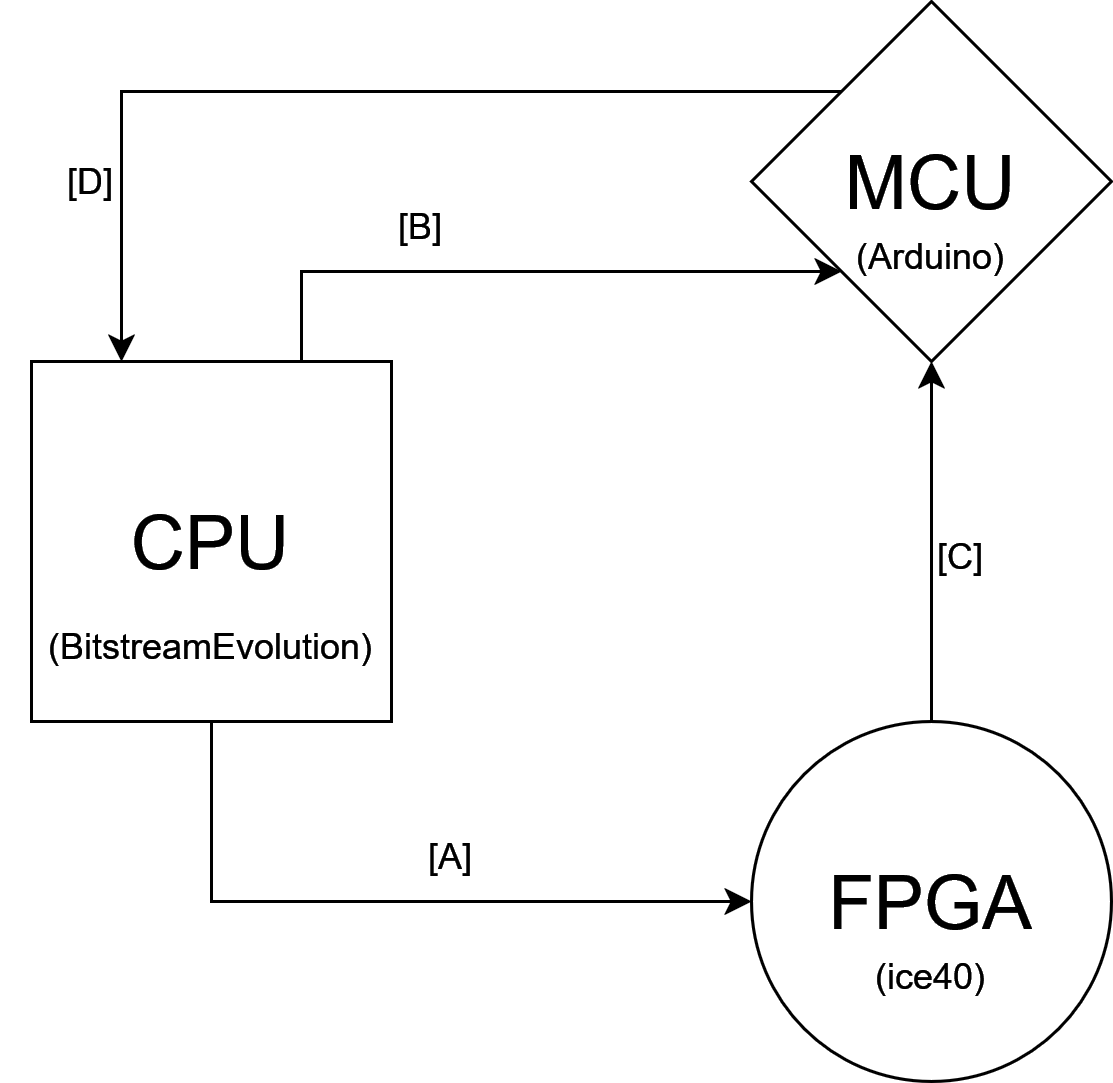
\includegraphics[width=2.5in]{figures/loyd1.png}
\caption{System Diagram}
\label{fig_sys_diagram}
\end{figure}




During evolution, the CPU generates and maintains a population of individuals (bitstreams). The CPU will compile these bitstreams and upload circuits to the FPGA, asking the microcontroller for readings. The FPGA readings are transmitted via direct wired connections to the microcontroller, which reads them and returns them to the host CPU. The host CPU will use the recorded data to determine an appropriate fitness score, run the evolutionary process according to configured parameters, and create the next generation for evaluation and modification.

\begin{figure}[!ht]
\centering
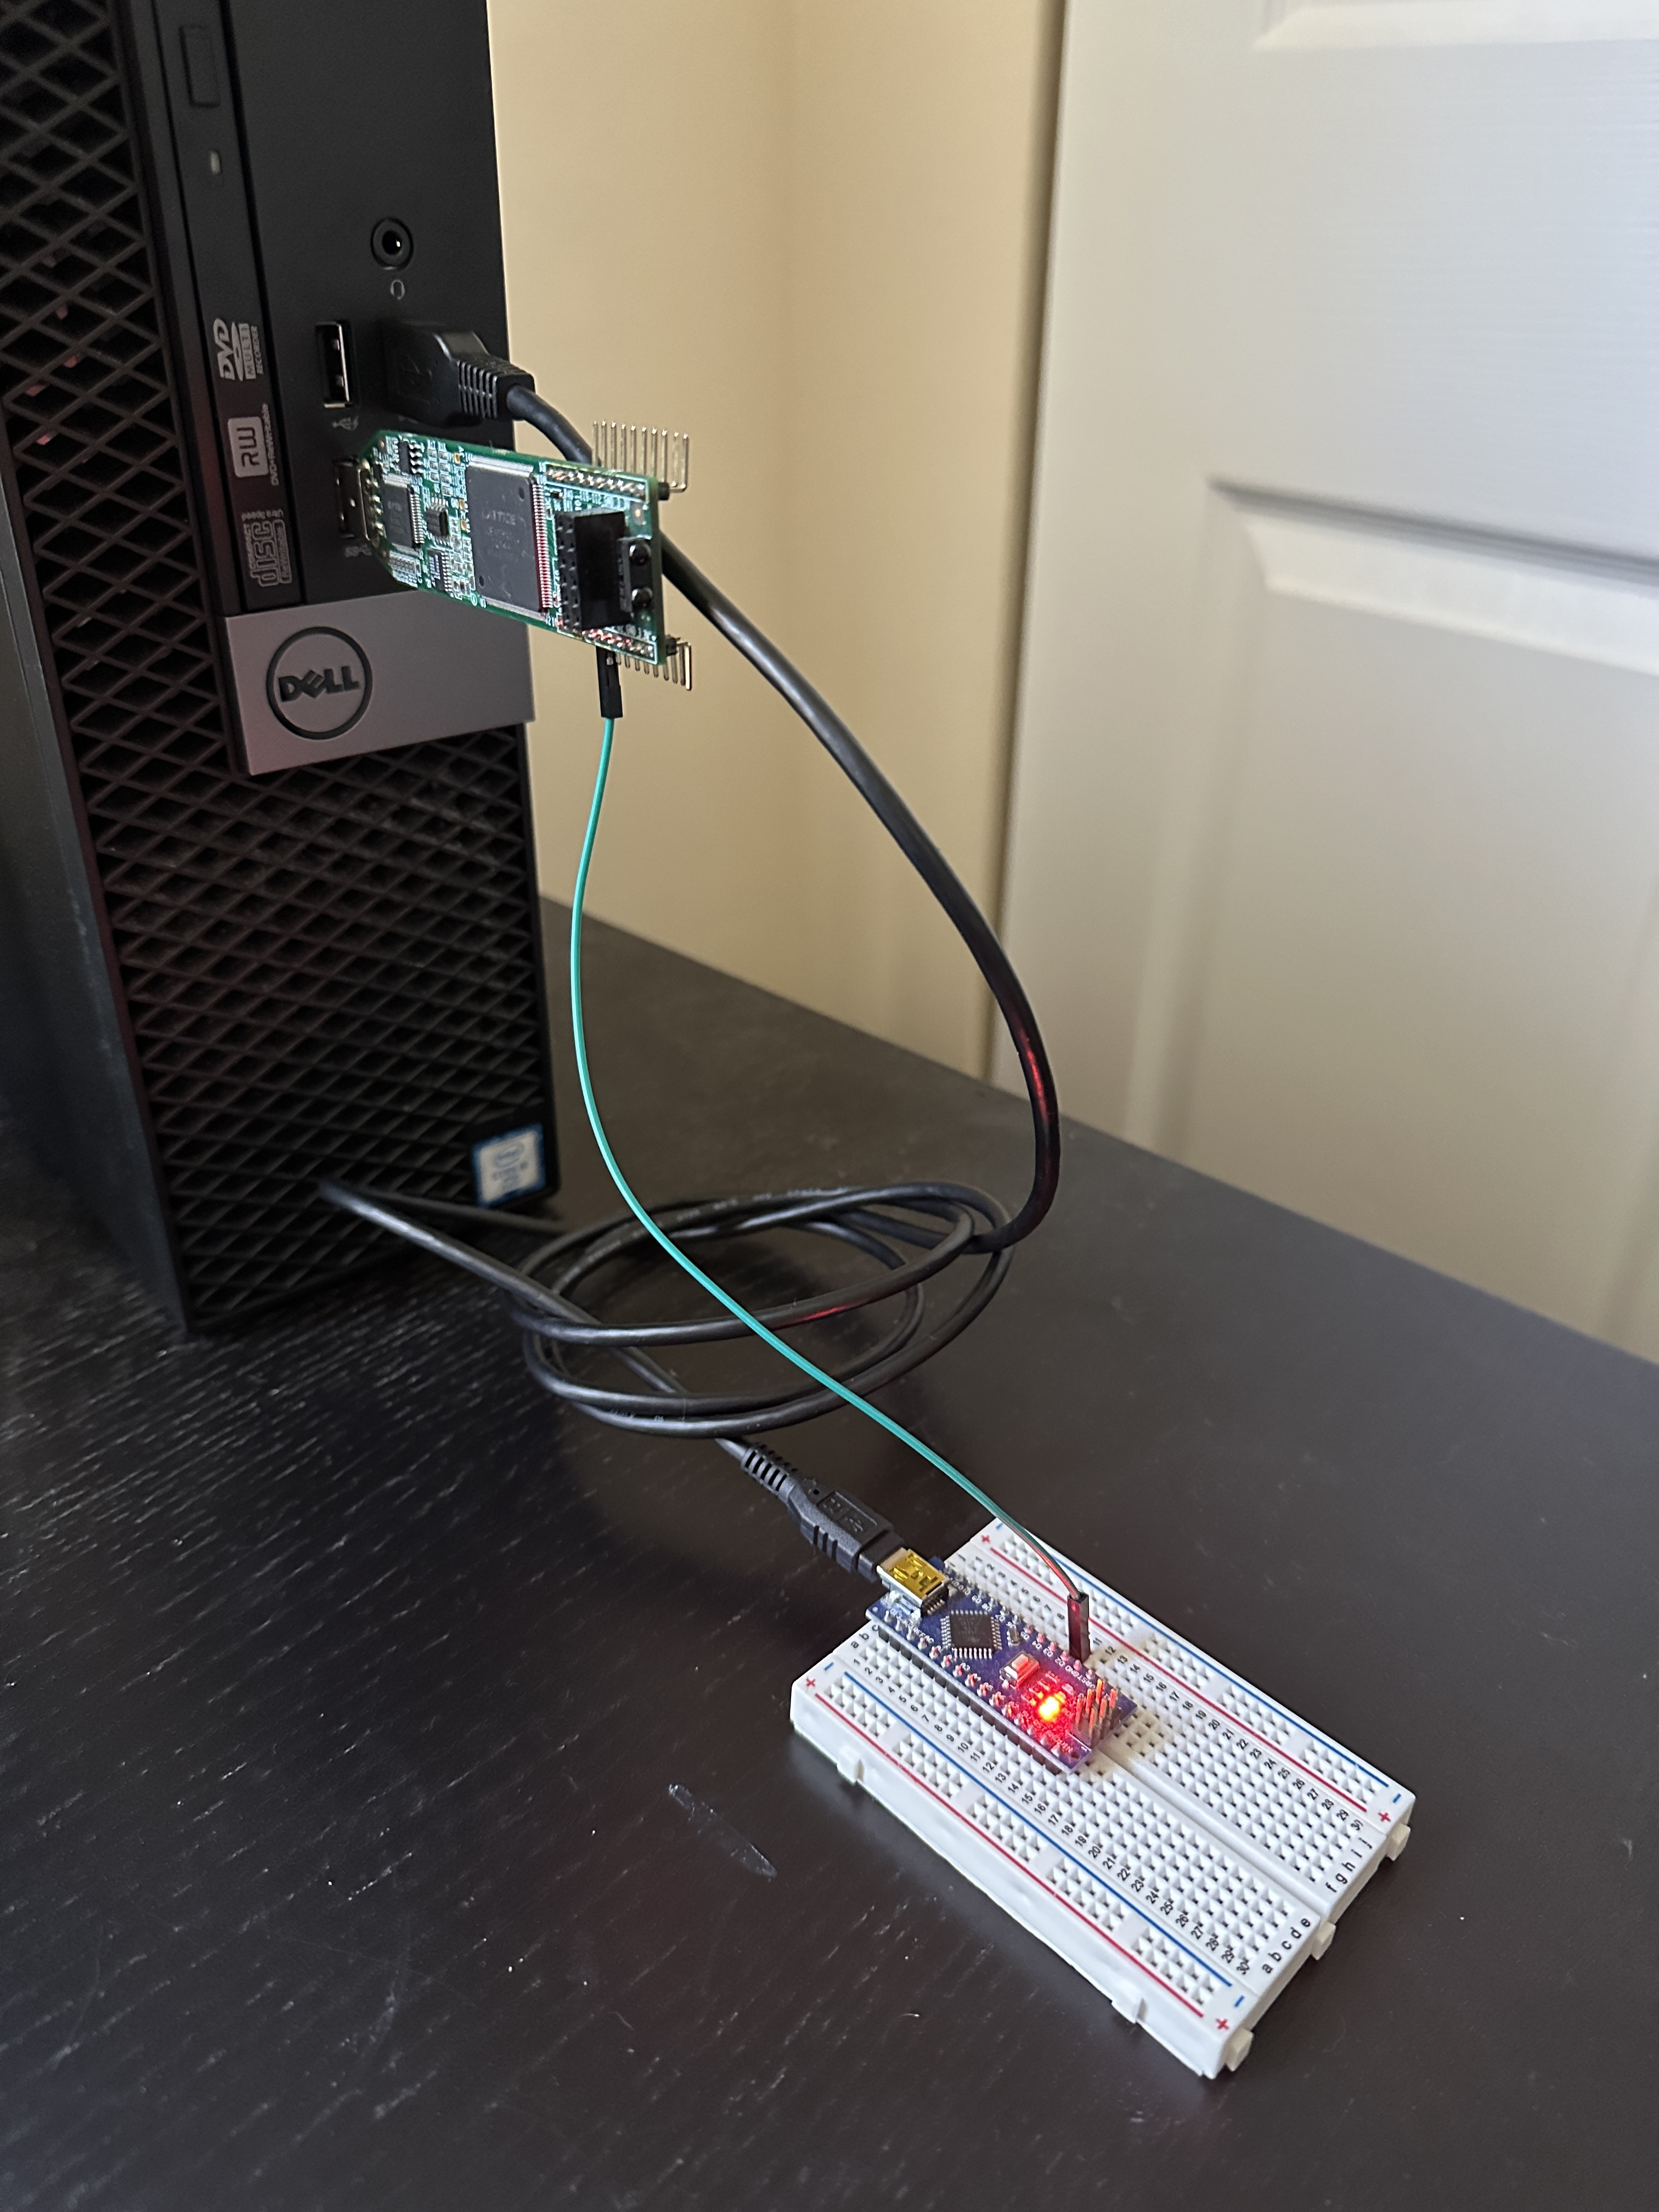
\includegraphics[width=2in]{figures/loyd2.JPG}
\caption{Hardware Setup for the System, including a desktop, iCE40 FPGA, and Arduino Nano connected via USB cables and a wire.}
\label{fig_hardware_setup}
\end{figure}

\subsection{Hardware}

Along with a host CPU, our system works with Lattice iCE40 HX1K FPGAs and Arduino Nanos which are shown in Figure \ref{fig_hardware_setup} \highlight{(both of which can be} \highlight{purchased online on sites such as digikey.com or store.arduino.cc)}. We have used the \href{https://www.latticesemi.com/icestick}{iCEStick Evaluation Kit} development board, but other platforms providing similar access to an iCE40 HX1K device should be compatible. Both the iCE40 HX1K and Arduino Nano were chosen for their low cost and common use in open-source tools. With Arduino boards, we can easily read and record analog or digital signals produced by the FPGA. Through the use of serial communication, these signals can be sent to the host CPU for analysis. 




\subsubsection{Lattice iCE40 HX1K FPGAs}
For the FPGA, Project IceStorm\cite{WolfProjectIceStorm} provides an open-source toolkit for analyzing and modifying the bitstreams of  circuits. These tools allow direct modification of the bitstreams of FPGAs. This opens the door for exploitation of the hardware (taking advantage of non-linear effects), with a set of defined components. 


In our experiments, we only modify the bits of the logic tiles. These bits control how the tiles are routed together and what function each tile performs. We restricted our experiments to only the modifications of bits in a contiguous block of 96 logic tiles. This is both due to the immense size of the search space (160 total logic tiles, each with 864 bits, for a total of 138,240 bits), and to get as close as possible to Thompson's original experiments, which utilized 100 logic tiles \cite{ThompsonAnPhysics}. The rows and columns in each tile that can be modified throughout evolution are controlled by a user-defined configuration. Additionally, the system supports multiple I/O configurations for the FPGA. 

Many settings were fixed across all the experiments reported on in this paper, and we provide example configuration files specifying these settings in the \href{https://github.com/evolvablehardware/BitstreamEvolution}{github code repository}. Examples settings include modifiable regions, the baud rate (115200) for the Arduino Nano, and the I/O pins. Finally, Project IceStorm provides support for converting the bitstream files (stored as ASCII characters for easy modification) into binary files for compiling and uploading.% to the FPGA.

\subsubsection{Increasing iCE40 FPGA Programming Speed}
Although not required to use our platform, there is a documented means of increasing the programming speed of the FPGA itself. Project IceStorm documents the process for this hardware modification, which involves jumping the S RAM chip. This allows for direct writing to the FPGA and using the $-S$ argument in the $iceprog$ tool. Writing directly to the FPGA means that the data is not stored in memory and thus will not be saved after a power cycle. Fortunately, this is not a problem for the system since we always reprogram the chip before we cycle power. The exact speed-up may vary based on local configuration, but in one of our test configurations, the time to program was reduced from about 9 seconds to 1 second. Instructions to make this modification can also be found on the public \textit{Bitstream Evolution} \href{https://github.com/evolvablehardware/BitstreamEvolutionHardware}{hardware repository}.



\subsubsection{Disabling  iCE40 FPGA Clock}
The clock on the FPGA is disabled in each of the experiments we report on. The purpose of this is to explore the capacity for evolution to discover circuits capable of generating signals at different timescales without relying on a clock. In addition to no clock signal, no input signal is directly provided to the FPGA as we currently focus on generative tasks. It is worth noting that disabling the clock allows for, and encourages, the possibility of the FPGAs picking up on an external signal in the environment and using that throughout evolution.


\subsubsection{Arduino Nano}
% TODO: introduce Nano, strengths (cost, common, documented) weakness (reliability)
The system uses Arduino Nanos as our primary way of receiving data from the FPGA. Nanos were chosen because of their low cost (less than \$25), expansive documentation, and ability to read both analog and digital signals without any additional hardware. During evolution, the CPU uses the serial interface to tell the Arduino when and what type of data to record. The Nano uses either its analog-to-digital converter (ADC) to record a circuit's waveform or digital interrupt pins to record logical transitions.
%a circuit's frequency. 
When recording the analog waveform, we take 500 samples, one every 10 microseconds, for a total sampling time of 5 milliseconds. When recording the number of pulses, we use one of the Arduino's interrupt pins to record the number of times the FPGA output %goes HIGH 
transitions from low to high
over an interval of 1 second. This data is then sent back to the CPU, using the serial interface, for further processing. We plan to extend support to include additional microcontrollers in the future. 


\subsubsection{Aliasing Issues with Arduino Nano}
\label{sec-nano-aliasing}
The primary limitation of the current approach lies in the overall accuracy constraints of the Arduino Nano. In this current version, since we are not filtering out signals that surpass the reading precision of the interrupt pin, we encounter the issue of signal aliasing. Specifically, certain signals may surpass our reading capability, and when attempting to read such signals the resulting data may be inaccurate. 


\begin{figure}
    \centering
    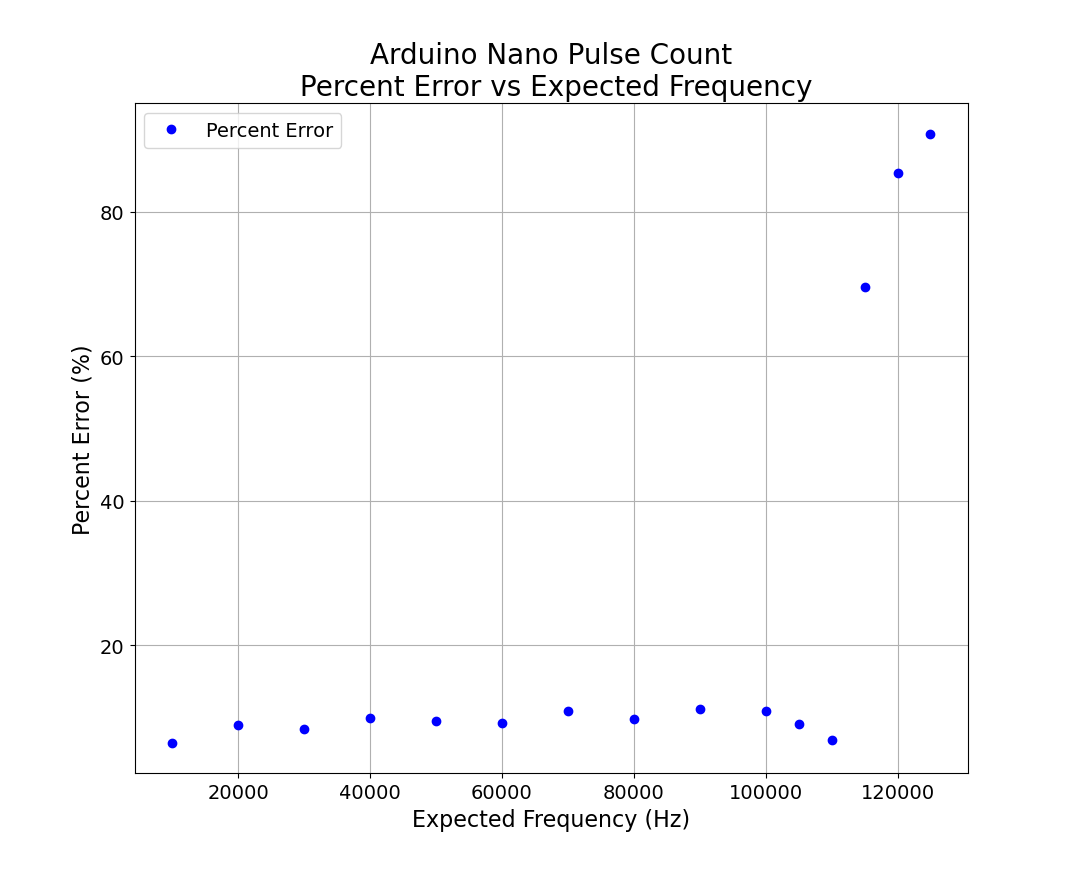
\includegraphics[trim= 30 20 0 30,scale=0.35]{figures/loyd3.png}
    \caption{Arduino Nano Interrupt Accuracy Graph. Showing the percentage error for the readings when a particular ground truth signal is provided as an input to be read.}
    \label{fig_interruptaccuracygraph}
\end{figure}



As seen from Figure \ref{fig_interruptaccuracygraph} anything over about 110 kHz is not accurate. Despite this, we can evolve an oscillatory circuit that will produce a certain interrupt report on an Arduino. However, in principle, this report could be caused by several different frequencies. For the oscillatory experiments we report on, although we targeted frequencies in the more accurate range of Arduino readings, there may be differences in the reported frequency measured and the underlying waveform. 

To combat these issues, we have considered adding a low pass filter between the Arduino Nano and the FPGA (Figure 1 [C]) to limit the frequencies being passed into the Arduino as only those within a sufficiently accurate measuring range as shown in Figure \ref{fig_interruptaccuracygraph}. %While in theory, this would make the results much more consistent, it would also both limit the overall range of frequencies we can evolve and would make the evolved circuit dependent on this low pass filter. However, this would ensure that the frequencies that are passed to the Arduino match the result we are reporting back to the evolutionary algorithm.
One alternative approach would be to use devices with greater accuracy, such as ESP32 microcontrollers.


% Notes for filter values 
% R = 160Ω
% C = 0.01uF
%

\subsection{Software}
%In this section, we focus on the ``CPU" component of the overall system. We begin with an explanation of software configurable evaluation modes, which allow for both intrinsic experimentation as well as testing of specific components of the system. Next, we discuss how fitness can be evaluated and the motivation behind the various fitness functions provided. We will summarize key features of the software, their purposes and how they are used.

In this section, we focus on the ``CPU" component of the overall system. We begin with an overview of the evolutionary algorithm to give context for specific features. Next, we discuss the population initialization settings and the different types of execution modes. Finally, we explain the methods of fitness evaluation and selection of successive generations.

\begin{figure*}[!t]
\centering
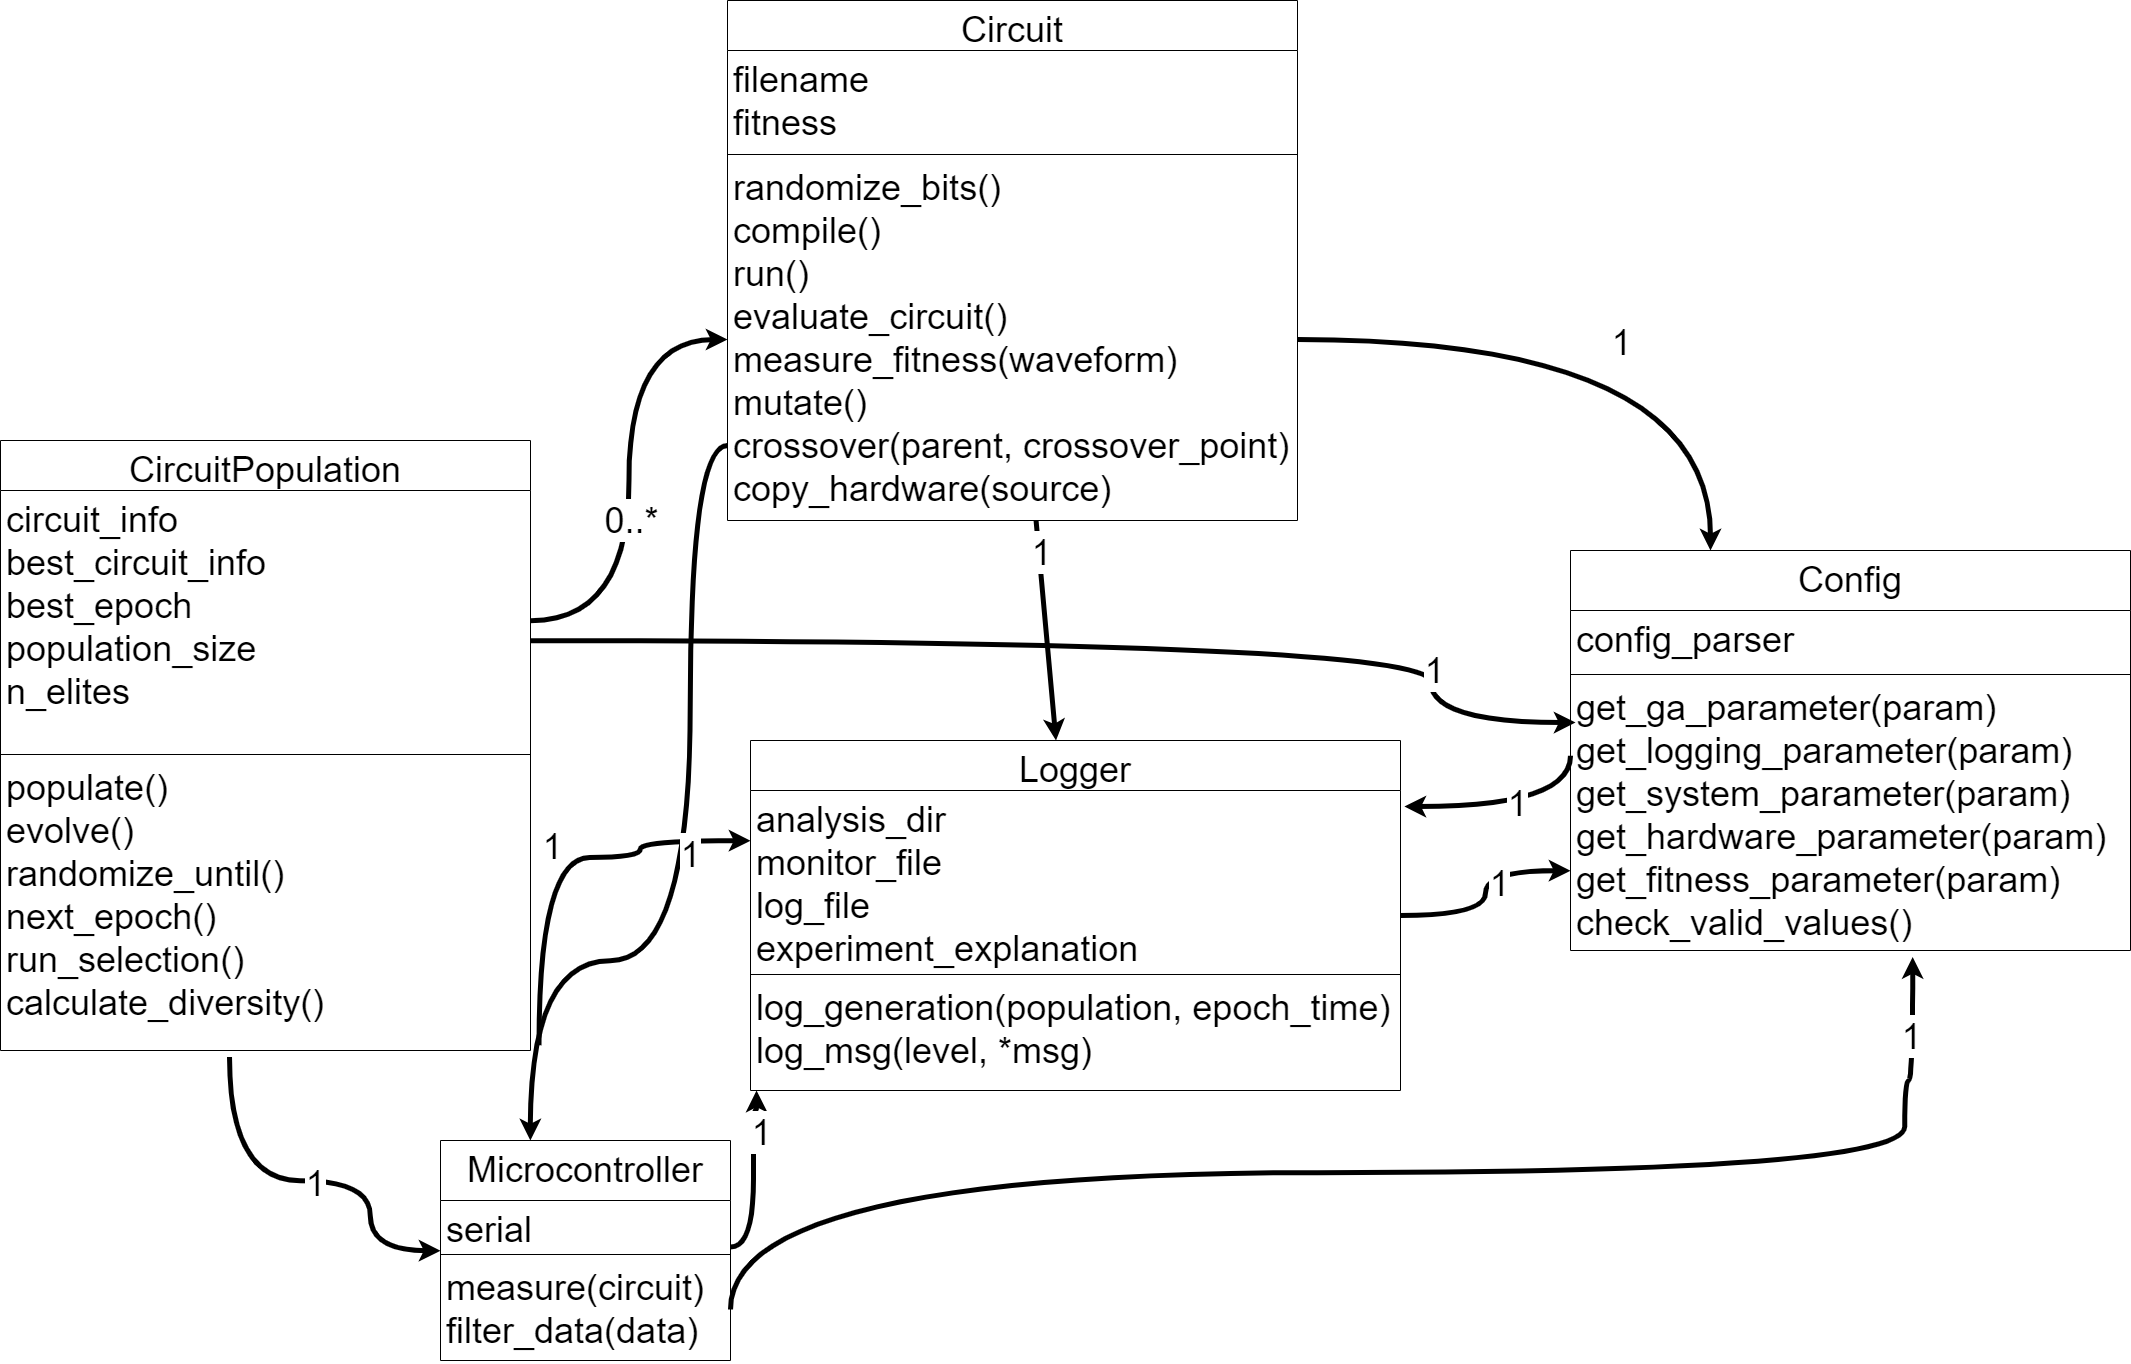
\includegraphics[width=6.4in]{figures/loyd4.png}
\caption{Class Diagram of the \textit{Bitstream Evolution} system}
\label{fig_uml}
\end{figure*}

% \begin{figure}[!b]
% \centering
% 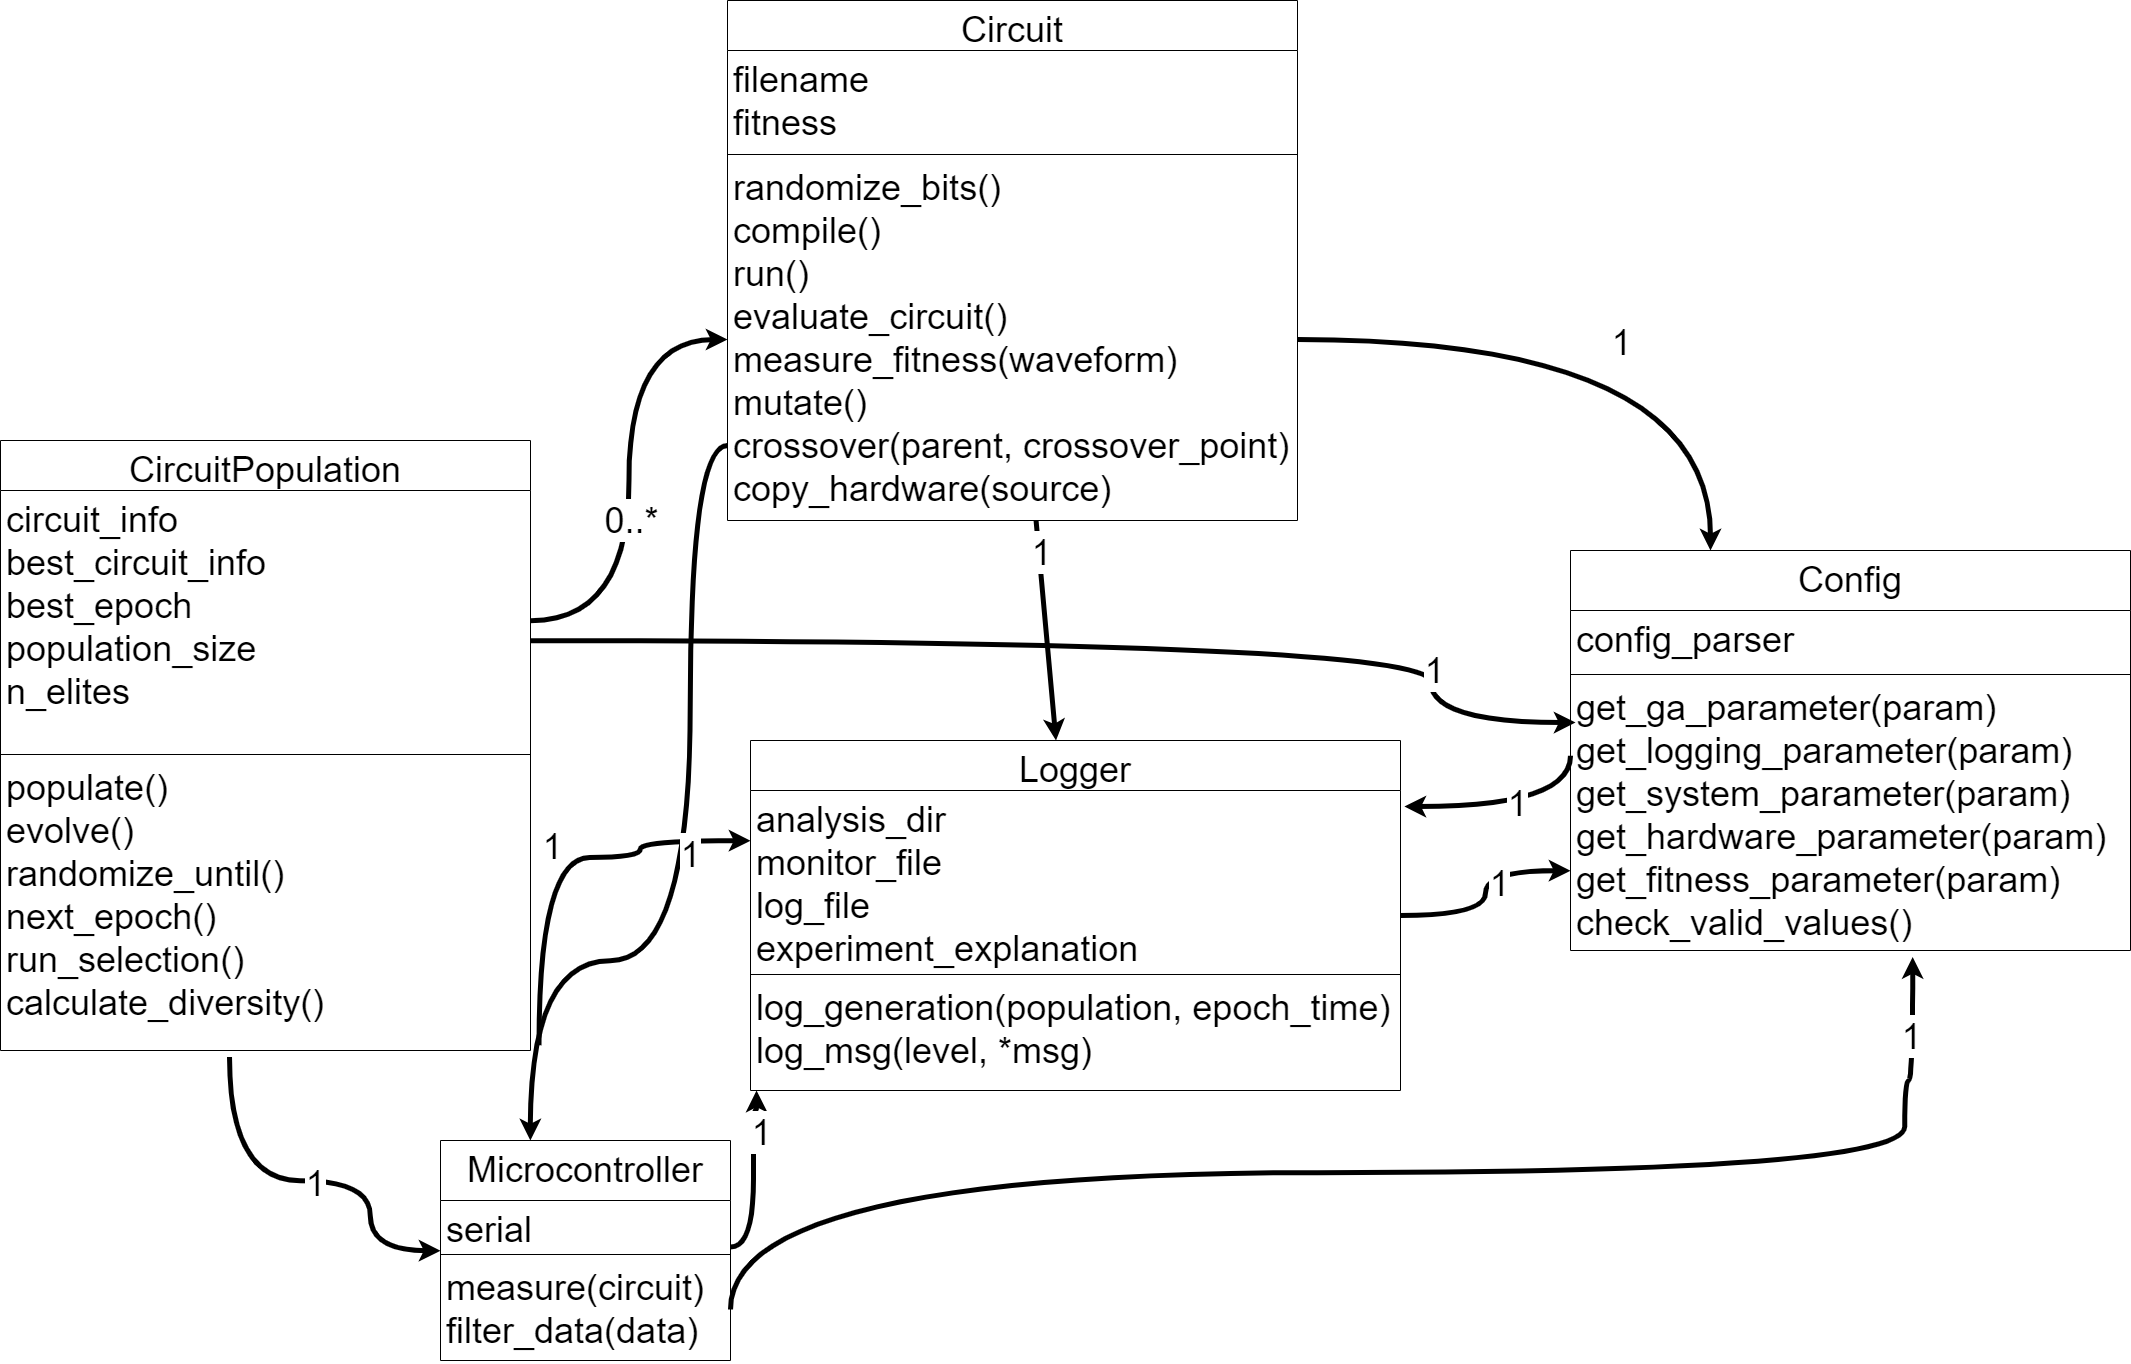
\includegraphics[width=3.4in]{figures/loyd4.png}
% \caption{Class Diagram of the \textit{Bitstream Evolution} system}
% \label{fig_uml}
% \end{figure}


\subsubsection{Evolutionary Algorithm}
The evolutionary process starts with initializing the population, which may start with randomization (see Initialization Modes). Figure \ref{fig_uml} provides a high-level design overview in the form of a class diagram. The population and evolutionary process is managed by the \texttt{CircuitPopulation} class. After population initialization, during each generation, the \texttt{CircuitPopulation} class checks if evolution should terminate. It then evaluates and sorts the \texttt{Circuit}s. Each \texttt{Circuit} instance is responsible for evaluating itself (see section \ref{sec_fitness-evaluation} and managing its own hardware file (performing mutations, crossover, etc). The microcontroller itself is encapsulated in the \texttt{Microcontroller} class, of which the program has a single instance that all other components share. The \texttt{Microcontroller} class is used to gather measurements for calculating fitness, which the \texttt{Circuit} does once it gathers its readings. Upon gathering fitness values, the \texttt{CircuitPopulation} performs selection (see section \ref{sec_selection_methods}), followed by mutation and crossover. At this stage, it injects random circuits if specified to do so. Finally, all plot data is updated, and the next generation begins.





\begin{table}[!ht]
\caption{Initialization Modes\label{tab:table_initmodes}}
\centering
\begin{tabular}{|c|c|}
\hline
\textbf{Mode Name} & \textbf{Simple Description}\\
\hline
RANDOM & Completely random bitstream \\
\hline
CLONE\_SEED & Clone the specified seed\\&circuit to fill the entire population \\
\hline
CLONE\_SEED\_MUTATE & Clone the specified seed \\&circuit to fill the entire\\&population, but also mutate it\\
\hline
EXISTING\_POPULATION & Clone an existing population  \\& from a specified directory \\& to  fill the entire population \\
\hline
\end{tabular}
\end{table}

\subsubsection{Initialization Modes}
Given the slow evaluation time of circuits, it is important to try to start with an initial population with its best chance of success. Based on different goals, different initialization methods may be useful, and we provide and explain several of them in this section. Table \ref{tab:table_initmodes} provides a high-level description for each of these methods.

The \textit{fully random mode} (RANDOM) will randomize all (modifiable) bits in each circuit of the starting population, offering the highest initial diversity. This may make sense to use when trying to evolve a circuit for the first time on a new task or new hardware.

The \textit{clone from seed} (CLONE\_SEED) option will use a seed individual circuit and make copies of it to create the entire initial population. This causes experiments to start with very low diversity but can be used to improve upon a known high-fitness solution. This may be useful when trying to continue an evolutionary run from either the same hardware or when measuring or testing transferability (see section \ref{transferability}).
%It also may be selected rather than cloning and mutating the seed circuit (see next variant) when the seed is unstable. Having additional copies also allows for more runs of the same circuit in the initial generations, raising the chance that at least one is able to reach a similar fitness to the original seed.

A similar variant is \textit{clone from seed and mutate} (CLONE\_SEED\_MUTATE), which will clone a seed individual but stochastically mutates each resulting circuit, raising the initial diversity while also building off of an existing solution. 

Both clone options can also be used to progressively guide evolution. For example, an experiment can be performed with one fitness function, and then the best individual can be taken and used to seed another experiment. This gives the initial population of this second experiment a place to start, without having to evolve a challenging task from scratch \highlight{(for example, running a variance-maximization experiment} \highlight{and using the resulting best circuit as a seed for an oscillator} \highlight{experiment)}

The \textit{existing population} (EXISTING\_POPULATION) option allows users to specify a directory that contains sub-directories of circuits that will be cloned and used as the initial population. This allows evolution to run on a previously saved population. This option may also be useful when exploring the transferability of circuits from one board to another.

The system also has randomization modes which aid in initialization, by randomizing circuits until they meet some criteria. 
%Circuits can be randomized until they meet certain criteria.
%variance fitness, pulse count, or get within a certain distance of a threshold voltage. 
This option can be configured to completely randomize circuits until they reach a certain goal, or mutate circuits, allowing the initialization setting to set the starting population. For example, one could start with an existing population and proceed to mutate circuits until reaching some criterion. Randomization can also be disabled to use the initialization mode to determine the starting population.



\subsubsection{Execution Modes}

\begin{table}[!ht]
\caption{Execution modes\label{tab:table_execmodes}}
\centering
\begin{tabular}{|c|c|}
\hline
\textbf{Mode Name} & \textbf{Simple Description}\\
\hline
INTRINSIC & Evaluates fitness on the FPGA \\
\hline
BITSTREAM\_SIM & Compiles bitstream and sums the bytes in the file \\
\hline
WAVEFORM\_SIM & Generates sine waves that can be treated\\&as an input signal \\
\hline
\end{tabular}
\end{table}


\textit{Bitstream Evolution} features different modes of bitstream evaluation, each 
modifying the behavior of the Circuit class, each of which is provided in Table \ref{tab:table_execmodes}.
%having different circuit behaviors. 
In the \textit{intrinsic} (INTRINSIC) mode, circuits are evolved and uploaded to the FPGA - this is the only intrinsic evolution mode. The other modes were introduced as methods of verifying and testing other parts of the system. 

The first true simulation mode, \textit{bitstream simulation} (BITSTREAM\_SIM) uses the files that are uploaded to the FPGA, but arbitrarily calculates fitness based purely on their bitstream (e.g. counting the number of 1s), rather than uploading them, for faster evaluation. This mode is useful for verifying that mutation and crossover are not corrupting the circuit files, and making sure circuits can be compiled properly. 


The other simulated mode, \textit{waveform simulation} (WAVEFORM\_SIM) does not use circuit files at all, but rather it's own short, contained arbitrary bitstream. For this reason, every circuit in this mode will start with a default (all 0's) bitstream, unless the RANDOM initialization mode is selected (see Initialization Modes) --- this is because the waveform bitstream is only 100 bits, and using hardware files to seed the initial population is not applicable. In this simulation mode, circuits will generate waveforms weakly similar to the noisy signals output by the analog pins on the FPGA. This mode is useful for testing selection methods and the evolutionary loop, as it allows rapid simulation without any FPGA interaction.


\subsubsection{Fitness Evaluation}
\label{sec_fitness-evaluation}
Currently, there are three different fitness functions used to evaluate a circuit while in the fully intrinsic mode: variance maximization, sensitive pulse count, and tolerant pulse count. Table \ref{tab:table_fitnessfunctions} provides a simple description of each and the equations are provided below. The variance and pulse count fitness functions are not comparable. We chose to use different types of functions to highlight the system's ability to evolve circuits suited for a wide range of tasks.

\begin{table}[!ht]
\caption{Fitness Functions\label{tab:table_fitnessfunctions}}
\centering
\begin{tabular}{|c|c|}
\hline
\textbf{Function Name} & \textbf{Simple Description}\\
\hline
VARIANCE & Evaluates the ``noisiness" of a\\&waveform \\
\hline
SENSITIVE\_PULSE\_COUNT & Evaluates the closeness of the\\&recorded pulse count to the\\&desired frequency,\\&with fitness decaying rapidly\\&as distance from the\\&target frequency increases \\
\hline
TOLERANT\_PULSE\_COUNT & Evaluates the closeness of the\\&recorded pulse count to the\\&desired frequency,\\&with fitness decaying less\\&rapidly as distance from the\\&target frequency increases\\
\hline
\end{tabular}
\end{table}

\begin{equation}
\label{fitness_variance}
\Psi = \frac{\sum_{i}^{N} {(|x_i - x_{i+1}|)}}{N}
\end{equation}

\begin{equation}
\label{fitness_pulse_sensitive}
% \Psi = \frac{1}{|f - n|}
\Psi = \begin{cases}
        \frac{1}{|f - n|} & \text{if } n > 0\\
        0 & \text{otherwise}\\
        \end{cases}
\end{equation}


\begin{equation}
\label{fitness_pulse_tolerant}
% deviation = 0.025 * desired_freq # 25 for 1,000 Hz, 250 for 10,000 Hz
% fitness = math.exp(-0.5 * math.pow((pulses - desired_freq) / deviation, 2))
% \Psi = e^{-0.5 (\frac{f-n}{0.025*f})^2}
\Psi = \begin{cases}
        \exp(-0.5 (\frac{f-n}{0.025*f})^2) & \text{if } n > 0\\
        0 & \text{otherwise}\\
        \end{cases}
\end{equation}


The first fitness function, \textit{variance-maximization} (VARIANCE, equation (\ref{fitness_variance})) focuses on maximizing the ``noisiness" of the waveform. It takes the sum of absolute differences between consecutive points of the waveform ($x_i,x_{i+1}$) read in at discrete time steps, and divides that by the number of voltage readings ($N$). This means the measure of ``noisiness" is the average difference between voltage readings on consecutive time steps. Since the circuit's waveform may vary each time it is measured, this fitness function is stochastic. However, as discussed in section \ref{sec_results_sensitivity}, the fitness tends to stay relatively consistent across trials in the same environment. For each evaluation, we take 500 samples delayed by 10 \si{\micro\second} each, for a total sampling window length of 5 \si{\milli\second}. 

To evolve oscillatory circuits that produce rising-edge pulses at a given frequency, we have developed and utilized two different fitness functions (sensitive and tolerant pulse count). We have also made adjustments to them to improve the quality and rate of evolved circuits. Each fitness function attempts to match the number of times ($n$) the waveform rises above a threshold voltage over a span of a second with a desired frequency ($f$), however, the sensitive function is more punishing towards measurements away from the target frequency, as discussed later in this section. We count pulses using the Arduino's digital interrupt pin over a sampling window of one second. Thus, the pulses counted is the frequency of the circuit. 



% timeout issue
\subsubsection{Addressing Hardware Timeout Issues with Software}
One technical difficulty we discovered is that occasionally when evaluating a circuit, the Arduino receiving the signal from the FPGA would timeout, meaning that no result was returned to the CPU. This does not indicate that zero pulses were recorded, but rather that the Arduino never delivered a response. Our working hypothesis is that this may happen when a circuit produces so many rising edges that it continually interrupts the Arduino, thus preventing it from executing its return result commands. Although this might be addressed by changes in hardware (see section \ref{sec-nano-aliasing}), we elected to address this issue in software by recording such non-responsive behaviors as producing $-1$ pulses for the purpose of computing fitness \highlight{(to distinguish from a true result of 0 pulses)}.  If we do encounter a timeout, we attempt to get the data five additional times before moving on and assigning a pulse reading of $-1$. 



\subsubsection{Encouraging Non-Zero Pulse Counts}
% 0 pulses closer to target
A second issue we discovered was that when targeting certain frequencies, evolution would converge on circuits that produced zero pulses. Upon further investigation, we recognized that evolution would discover circuits with non-zero pulse counts, but in many cases these circuits would produce a frequency much higher than that. Under these circumstances, when the conventional fitness function (\cite{Thompson1998OnEvolution,Whitley2021ResurrectingHardware}) was targeting a relatively low frequency (under 20 kHz), a circuit producing \textit{zero pulses} would receive a \textit{higher} fitness score than a circuit producing \textit{a large number of pulses}.

Further compounding this issue is that we have found it very difficult to produce non-zero pulse counting circuits when randomly generating circuits. To address this we normally initialize the population with one or more seed circuits that have demonstrated a positive number of pulses. Although genetic drift \textit{might} eventually arrive at a non-zero pulse counting behavior, this is not necessarily efficient, which is a concern given the exceedingly long evaluation time of each circuit. For this reason, we decided it would be best to reward circuits for \textit{any} non-zero pulse counting behavior.

% +1 bonus
Based on these challenges, we created a fitness function (SENSITIVE\_PULSE\_COUNT, equation (\ref{fitness_pulse_sensitive})). This was derived from past work \cite{Whitley2021ResurrectingHardware} and was adjusted to incentivize selection for positive pulse counts \highlight{(we temporarily added a $+1$ bonus to circuits that achieved any positive number of pulses, but subsequently determined this was unnecessary and simply assigning a fitness value of 0 to both circuits that caused a timeout issue or produced 0 pulses was sufficient; this would have had a marginal effect on the results and in cases where it was present, we recalculated fitness values for any data presented to compensate for the adjustment).}
%We added a $+ 1$ bonus to reward circuits that produce any positive number of pulses, as compared to those that produce zero pulses or cause the timeout issue (recorded as -1 pulses) discussed earlier.

%This feature was added late in development, so some of the results presented feature the old fitness evaluation scheme without the bonus. This will not have a substantial impact on the takeaways from results reported in this paper, which should be qualitatively similar with or without this bonus. Fitnesses from experiments performed with the bonus have been recalculated using the raw pulse count measurements, to standardize all fitness measures reported.






\subsubsection{Increasing Tolerance to Frequency Variation}

In the original fitness function from \cite{Whitley2021ResurrectingHardware} and to a lesser extent this one, if a circuit was even one Hz off the desired frequency, its fitness would be dramatically reduced (hence, our name of \textit{sensitive} pulse count function). This could lead to circuits with similar behavior having wildly different fitnesses. When using fitness proportionate selection (see \ref{sec_selection_methods}), this could lead to one circuit being over-selected and wiping out most of the existing population. Normally, this is not much of a concern, but because of the stochastic nature of the fitness function and inaccuracy of the Arduino there is a possibility of a single ``lucky" but unreliable circuit was concerning. Given the occasional population crashes (sudden plummet of best and average fitness) that we had observed, we wanted to try to address this possible issue.

To counteract this, we added a second oscillator function (TOLERANT\_PULSE\_COUNT, equation (\ref{fitness_pulse_tolerant})). This one uses exponential decay to help smooth the fitness distribution around the desired frequency. In a case where the desired frequency is 50k Hz, and a circuit produces 49,999 pulses, the sensitive pulse count fitness would be 1.5, while the tolerant pulse count fitness would be 1.99999968.  Thus, we are attempting to account for the stochastic nature of our circuit evaluations by introducing more tolerance into fitness functions. However, in our experiments, we have not found a significant difference in the rate of evolution in the two functions, as discussed in section \ref{sec_pulse_count_results}. Identifying causes of population crashes and a more rigorous comparison of these two fitness functions remains an area for future investigation.








\subsubsection{Multiple Samples and Passes}

Both of the pulse count fitness functions support the ability to do multiple samples of each circuit or multiple passes through every generation. The system does support this for all our fitness functions, but the system currently assumes each of the samples have a fitness between 0 and 2, while the variance maximization fitness for a single sample can be above 300. We have not found a need to conduct circuit variance maximization experiments with multiple samples and passes. This is because circuits' variance maximization fitness measures are much more consistent than the pulse count fitness measures. Thus, there is a less need to encourage consistency when evolving circuits for variance maximization. When doing $i$ samples, each circuit is tested $i$ consecutive times. When doing $j$ passes, every circuit in the generation is tested one after each other, and then this process is repeated $j$ times. It is possible to do both multiple samples and passes in the same experiment. This results in a total of $i \times j$ measurements per circuit. The product of the measurements is used for fitness calculation (all measurements are in the range of 0 to 1). This product is taken before the additional fitness boost is given. In this case, the fitness boost (+1) is given if any of the samples of passes of a circuit record 1 or more pulses. We chose to use multiplicative aggregation (as compared to averaging or taking the minimum) to further encourage consistent circuits to be evolved. This also helps address the issue discussed in the previous section of unreliable circuits being selected due to ``lucky'' evaluations.

Both multiple sampling ($i>1$) and taking multiple passes ($j>1$) are means of improving the consistency of individuals. The data for each pass is multiplied together (taking the lowest fitness from each sample batch), meaning multiple low-fitness readings are compounded, while one low-fitness reading will still have a large impact on an otherwise fit individual. Taking multiple samples is a simpler and faster way to record more measures than taking multiple passes. However, taking multiple passes will ensure a much larger time window in between each measure (or set of measures) being taken, giving more time for the environment to change. This aims to give circuits a harder time incorporating volatile environmental factors into their function, although taking $i$ passes takes longer to run than taking $i$ samples since circuits must be re-uploaded to the FPGA for each pass, while they only need to be uploaded for the first of the $i$ samples.


\subsubsection{Selection Methods}
\label{sec_selection_methods}

\begin{table}[!ht]
\caption{Selection Methods\label{tab:table_selectionmodes}}
\centering
\begin{tabular}{|c|c|}
\hline
\textbf{Selection Method} & \textbf{Simple Description}\\
\hline
Fractional Elites Tournament & A set of circuits are defined as elite. \\& Elite and non-elite circuits are paired\\& such that non-elites get replaced \\
\hline
Fitness-Proportionate & Circuits' chances of being selected\\&is proportionate to their fitness \\
\hline
Rank-Proportionate & Circuits' chances of being selected\\&is proportionate to their fitness rank \\
\hline
Classic Tournament & Circuits are repeatedly paired up\\&and evaluated, with the \\&higher-fitness circuit surviving.\\&Elites are excluded from the tournament. \\
\hline
Single-Elite Tournament & Same as classic tournament,\\&but only one elite \\
\hline
\end{tabular}
\end{table}

To select circuits for each next generation, there are five selection methods, which are fractional elites tournament, fitness- and rank-proportionate, classic tournament, and single-elite tournament which are accompanied with a simple descriptions in Table \ref{tab:table_selectionmodes}. These selection methods were implemented primarily with the goal of keeping elitism high, since small changes to circuits can dramatically reduce their fitness. Thus, it is important not to mutate every circuit in the population, or else we risk losing the progress made during evolution. This is primarily accomplished by using tournaments in our selection method. Each tournament has a size of two, and only the worst-performing circuit is modified.


In addition to our selection methods, each run may use single-point crossover. Single-point crossover restricts the number of changes that are made to one circuit, while uniform or multi-point crossover would likely disrupt many of the FPGA’s connections between logic tiles and functions and thus greatly reduce the circuit's fitness. Additionally, since the fitness evaluation is stochastic, a typically well-performing circuit might do poorly in one generation and be eliminated from the population. With high elitism, there is a greater likelihood this circuit will continue to be included (via duplicate copies) in the population. With many duplicate or similar copies in a successive generation, a particular circuit that has been successful in the past and has a bad run can be removed during selection without a complete loss of the circuit, which lives on through its clones.



Fractional elites tournament selection (Alg. \ref{alg-fractional-elites}) starts by sectioning off a group of the fittest circuits (the elites) that will be kept the same in the next generation. For each non-elite circuit, a circuit is randomly selected from the pool of elites and the circuits' fitnesses are compared. Every non-elite will be involved in exactly one tournament, while an elite circuit could be involved in multiple tournaments. The algorithm outlines our process for how mutation and crossover occur on our circuits. This is a general way to ensure elitism remains high, while maintaining some diversity throughout the population. Every other selection method is based off this one, with modifications described below.


\begin{algorithm}[ht]
\caption{Fractional Elites Tournament Selection} \label{alg-fractional-elites}
\begin{algorithmic}[1]
    \State $P \gets \text{current population of circuits}$
    \State $N \gets \emptyset$
    % \State $n \gets$ the number of elites
    \State $E \gets \{ \text{the best $n$ circuits} \}$

    \For{c, a non-elite circuit}
        \State $r \gets$ a random choice from $E$
        \If{ $\random (0,1) \leq \text{crossover probability}$}
            \State $c \gets$ crossover from $r$ to $c$
        \Else
            \State $c \gets r$
        \EndIf
        \State $N \gets N \cup \{\mutate(c)\}$
    \EndFor
    \State \Return $N$ as the new population
\end{algorithmic}
\end{algorithm}

Fitness-proportionate selection functions similarly to fractional elitism; the only difference is in the probabilities of each elite circuit being selected for comparison. Here, the probability of a random elite being chosen for any given tournament is its fitness divided by the sum of all the elites' fitnesses - i.e. Roulette Wheel selection. Again, each non-elite circuit is involved in only one tournament.

% Note: The above (fitness proportional) matches every circuit with an elite, performs either crossover or a direct clone, and then mutates. Same for rank proportionate

In rank-proportionate selection, the probability of an elite circuit being selected is based on its rank in the population instead of fitness. This generally keeps more diversity in the population, since having one extremely fit circuit with fitness proportionate selection means most of the next generation will end up with bitstreams similar to that circuit.



In single-elite tournament selection, only the best circuit in each generation is selected to be an elite, but otherwise works the same as fractional-elite tournament selection. This selection method is used when diversity in the population is prioritized, as only one circuit is kept the same from one generation to the next.


 For classic tournament selection, two circuits are randomly selected for the tournament at a time, without repetitions. The circuit with the higher fitness is treated as the elite. Using a tournament size of two (the only size the system currently supports), half the population is kept the same from generation to generation. This is most useful when we want to have a relatively stable population that minimally changes from one generation to the next. This method was inspired by the Microbial Genetic Algorithm \cite{Harvey2011TheAlgorithm}.

 \section{Illustrative Results}
\label{sec_results}

In this section, we report on experiments that can be easily run with the \textit{Bitstream Evolution} platform and illustrate the insights that can be gained in doing so. \highlight{These are not meant to be complete, comprehensive studies, but instead a demonstration of preliminary results that can be obtained using the Bitstream Evolution system.} We first report on the results of running experiments with the target frequency fitness function, which aims to evolve oscillatory circuits matching rising edge signals to a specific frequency. Second, we report on the results of transferring and evolving circuits for both the target frequency and the variance maximization fitness functions. Finally, we report on the results of fitness sensitivity analysis in which we explore the variability of fitness of single circuits repeatedly evaluated in the same physical configuration to assess robustness.


\subsection{Pulse Count Target Comparison}
\label{freq_cmp_section}

\begin{figure*}[!ht]
\centering
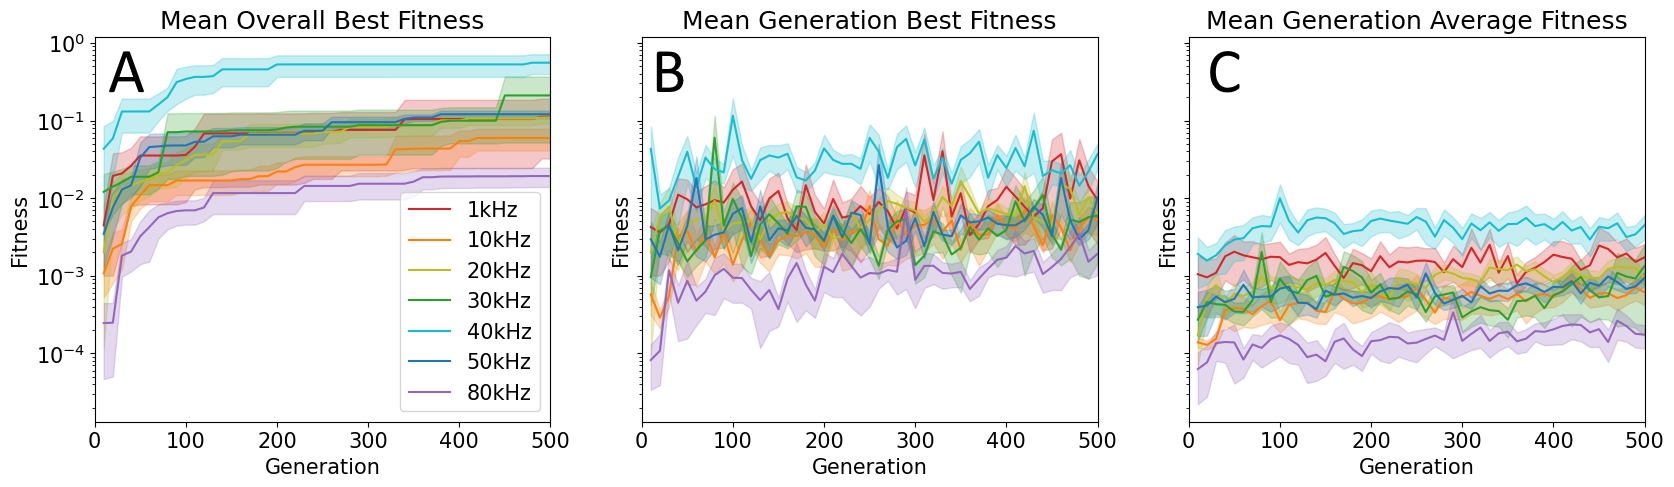
\includegraphics[width=7.1in]{figures/loyd5.png}
\caption{Overall Best, Generation Best, and Generation Average Fitness for different target frequencies, taken every 10 generations}
\label{freq_cmp}
\end{figure*}




One of the core challenges of evolvable hardware from its outset is bridging the timescales of signals in the biological and electronic domains. Because of the advances in the manufacturing of physical components (e.g. wire and transistor sizes) of electronics in the last twenty years, results from Adrian Thompson's work required demonstration of feasibility on modern hardware, which was done in \cite{Whitley2021ResurrectingHardware}. However, there remains an open question of evolution's ability to find circuits capable of operating at varying timescales.


To gain insight into the relationship between timescales and the evolvability of circuits, performed experiments comparing the evolution of (oscillatory) circuits targeting different frequencies. We hypothesized that generally higher frequencies would be easier to evolve than lower frequencies because the rate of propagation of electric signals is so high. During initial experimentation, we often observed randomly generated circuits starting with a frequency of around 40 kHz. Because of this, we decided to explore a range of target frequencies above and below this rate, \highlight{with experiments that varied only in the target frequency}. \highlight{Due to the time it takes to run these experiments, and our desire to test a range of target frequencies well above and well below 40kHz, we selected seven target frequencies that are a great distance from each other.} For each of the seven target frequencies in Figure \ref{freq_cmp}, we performed six experiments (on a mix of five different FPGAs), and averaged their results. The means across experiments are reported, specifically A) the best fitness reached by any circuit at any point during an experiment, B) the best fitness of the current generation, and C) the average fitness of the current generation appear in the figure.


The 40 kHz experiments consistently outperformed the others in each metric. The generation best (Figure 5.B) for the 40 kHz experiments was often on par with the overall best (Figure 5.A) for other frequencies, and the generation average (Figure 5.C) was generally on par with the generation best (Figure 5.B) for the other frequencies. In all metrics, the performances of different frequencies compared to each other are mostly consistent; for example, 80 kHz experiments performed the worst by every metric, and the 1 kHz, 20 kHz, and 50 kHz were often close together. This data suggests that some frequencies are easier to evolve than others. But, it's not purely based on proximity to a specific frequency, nor that higher frequencies are easier to evolve; the 30 kHz and 50 kHz experiments were similar to both the 1 kHz and 20 kHz experiments. 


One might suspect that an 80 kHz oscillator would be ``easy" to evolve if a 40 kHz is easily evolved given that it is exactly double that of 40 kHz. Such a solution might be possible if the same signal that is producing the 40 kHz signal is simply introduced into a parallel circuit that triggers the pulse twice as often. However, the 80 kHz experiments perform the worst out of all the targets, so the mathematical relationship between target frequencies may not be significant.


The progression of the best overall fitness of the various oscillators is very similar. It looks like the final overall best fitness is strongly correlated by the starting point. 
%All experiments made similar progress with their overall best, but the 40kHz oscillator had an initial fitness far above the others which was its biggest advantage. 
We suspect that the FPGAs are utilizing an environment-specific signal that makes 40 kHz an easy frequency to evolve for. Because these experiments have been performed on a variety of FPGAs in a variety of environments, we can rule out minute manufacturing differences and most environmental signals, as these are not likely to be common between all setups. The factors that could contribute would then be those that are common between all setups --- such as the microcontrollers, which are all the same model. More work is needed to determine the exact cause of this phenomenon. Another direction of future work is comparing the structure of the produced circuits across the different experiments.

\subsection{Transferability}
\label{transferability}



We also ran experiments to explore how circuits can adapt when being transferred from one FPGA to another during evolution. To do this, we started from a random population of circuits, evolved them on one FPGA for 200 generations, switched to a different FPGA and evolved on that one for another 200 generations, and then continued to switch back and forth. These experiments used a population size of 50 and completed 800 total generations.

The \textit{Bitstream Evolution} system allows the user to specify any transfer interval (TRANSFER\_INTERVAL) to control how quickly evolution switches between two FPGAs. To accomplish this, two FPGAs need to be plugged into the CPU and connected to a single Arduino Nano. The system will automatically handle the switching process. Because of this, the circuits can all be evolved in a relatively constant environment. The temperature, humidity, and other features of the test site can fluctuate throughout the experiment, but by having the system automatically switch between FPGAs, we can help limit the number of changes that occur from one transfer interval to the next. By limiting the changes in the external environment, we can focus on how minute hardware differences between FPGAs affect the behavior of circuits. 
% In comparison, for previous experiments, we would manually switch out the FPGAs between intervals, which meant hours or days could pass in between. This could lead to dramatic environmental shifts occurring during the experiment.

\subsubsection{Variance Maximization Circuit Transferability}
\begin{figure}[!t]
\centering
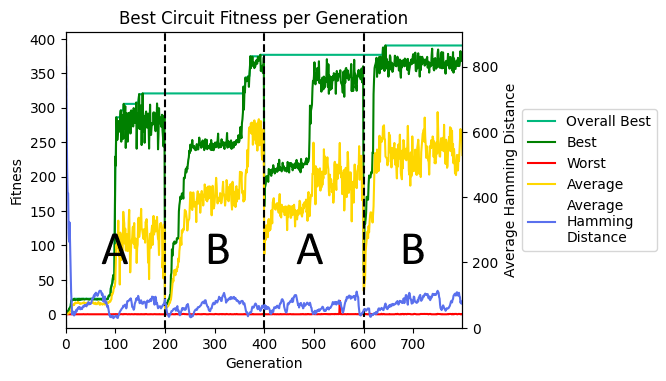
\includegraphics[trim= 10 0 0 0,scale=0.5]{figures/transferability/loyd6.png}
\caption{Fitness of circuits throughout an experiment exploring \highlight{the transferability of a }circuit evolved for the max variance fitness function. Evolution
occurs while alternating between FPGA ‘‘A" and ‘‘B" every 200
generations, as depicted in the plot.}
\label{fig_var_transferability_main}
\end{figure}

\begin{figure}[!b]
\centering
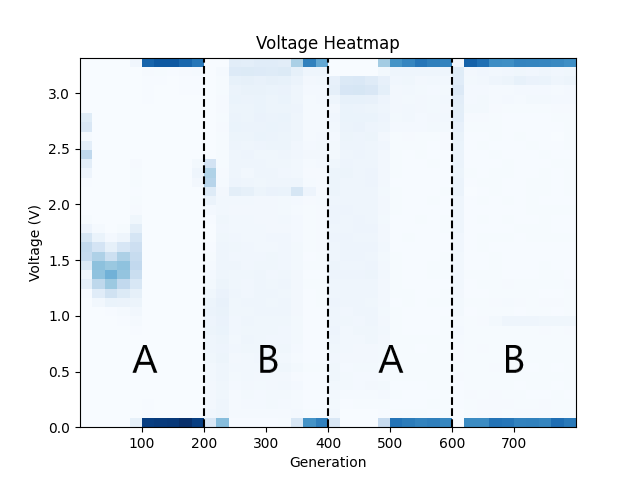
\includegraphics[trim=20 0 30 0,width=3.4in]{figures/transferability/loyd7.png}
\caption{This heatmap (with darker colors indicating higher frequency) shows the voltages of the best circuits throughout an experiment exploring transferability of circuit evolved for variance maximization fitness. FPGA ‘‘A" and ‘‘B" are alternated every 200
generations, as depicted in the plot.}
\label{fig_var_transferability_heatmap}
\end{figure}

The variance maximization experiment (Figure  \ref{fig_var_transferability_main}) shows how transferring between FPGAs can lead to the population escaping from local maxima in the fitness landscape. In the first interval, a maximum fitness of 320.742 was achieved during generation 155. The population was then evolved on a different FPGA for 200 generations, before switching back to the original FPGA. Here, it was then able to achieve a greater fitness of 376.79 during generation 392. Not much progress was made past this, possibly because in all intervals the population evolved to have its best circuits oscillate quickly between the highest and lowest possible voltage levels produced by the FPGA (Figure  \ref{fig_var_transferability_heatmap}).


With every interval, the time it took to recover back to a high fitness decreased. We define recovery time as the number of generations to return to 95\% of the maximum fitness of the previous interval. For the first transfer, it took 155 generations to return to 95\% fitness, but the following interval took 110 generations, followed by only 22 generations. This shows that evolving circuits on multiple pieces of hardware can help make them more adaptable to changes in their environment, with circuits quickly recovering from being transferred. Additionally, this suggests that using a seed population from another experiment, even if the experiment was done on a different FPGA, can help get results faster than starting from a random population.
%However, this may increase the chance the population will get stuck in a local maximum since there will be less diversity in the population. 

\subsubsection{Oscillator Transferability}
\begin{figure}[!t]
\centering
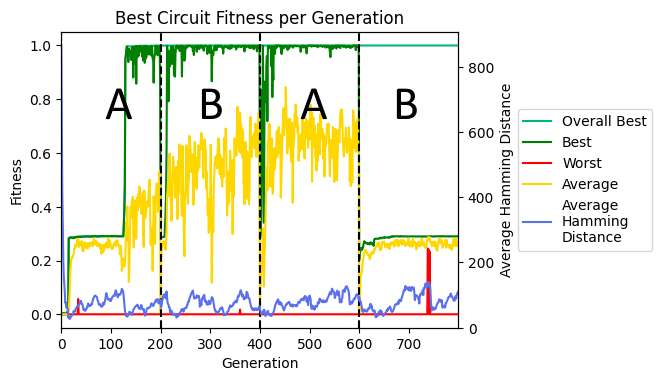
\includegraphics[trim= 10 0 0 0,scale=0.5]{figures/transferability/loyd8.png}
\caption{Fitness of circuits throughout an experiment exploring transferability of oscillators targeting an 80 kHz frequency. Evolution occurs while alternating between FPGA ``A" and ``B" every 200 generations, as depicted in the plot.}
\label{fig_pulse_transferability_main}
\end{figure}

\begin{figure}[!b]
\centering
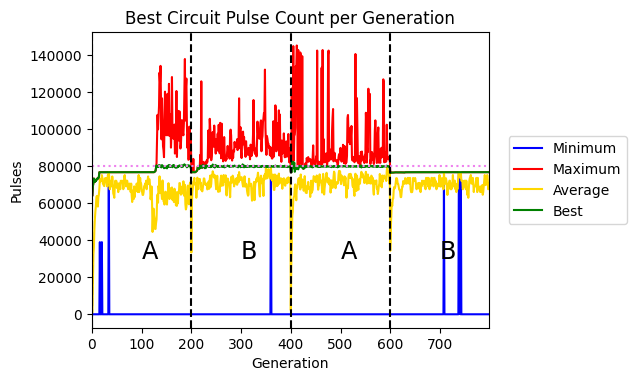
\includegraphics[trim= 10 0 0 0,scale=0.55]{figures/transferability/loyd9.png}
\caption{Produced frequencies of circuits throughout an experiment exploring transferability of oscillators targeting an 80 kHz frequency. Evolution occurs while alternating between FPGA ``A" and ``B" every 200 generations, as depicted in the plot.}
\label{fig_pulse_transferability_pulses}
\end{figure}

For testing the transferability of oscillators, we used our tolerant pulse count fitness functions (\ref{fitness_pulse_tolerant}), with a desired frequency of 80 kHz. Every circuit was sampled twice, and the worst measurement was used in fitness calculations. The purpose of using multiple samples was to evolve more consistent circuits. Our current recommended practice is to use fitness multiplication for multiple samples since it increases pressure on both consistency and quality.

This experiment (Figures \ref{fig_pulse_transferability_main} and \ref{fig_pulse_transferability_pulses}) shows many of the same traits of transferability as the variance transferability experiment. For one, the time it took the population’s best fitness to recover after a transfer point decreased throughout evolution. Additionally, the amount of the best fitness decreased by each transfer point also decreased for the first two transfer points. However, the last interval of generations saw significantly worse fitness than the previous intervals. Interestingly, the fitness was very similar to the fitness recorded in the first interval, despite being on a different FPGA. This means that transferability is not always effective.




\subsection{Fitness Sensitivity}
\label{sec_results_sensitivity}
In order to test how reliable our circuits are, we performed experiments taking single circuits and evaluating them repeatedly without making any changes to the circuit's bitstream. This helps us quantify how robust our circuits are when kept in a relatively stable environment. These circuits were tested in the same environment (same room and on the same hardware) they were evolved in, but differences in environmental factors, such as temperature and humidity, impacted the circuit’s performance. Since the circuits were not tested in a specially controlled room environment, this gives us the opportunity to see how robust they are to these small environmental changes.


\subsubsection{Pulse Count Sensitivity}
For these experiments, we ran pulse count experiments (see Appendix \ref{sec_pulse_count_results}) with a variety of desired frequencies. These experiments were run on three different FPGAs, all in differing environments. The best circuit of the final generation of each experiment was tested repeatedly for 24 hours straight following the canonical experiment. We conducted 10 of these experiments, with desired frequencies ranging from 30 to 90 kHz, in order to determine if different target frequencies led to different levels of consistency in the evolved oscillators. The correlation between the mean frequency recorded throughout each experiment and the standard deviation of frequency recorded in the trials in each experiment is $0.28509$. However, this could be due to the fact that a higher mean will naturally lead to a higher standard deviation than a lower mean. This is true even if most of the data points in each set are located within the same percentage of each mean. 

Because we consider such a wide variety of mean recorded frequencies in these experiments, it makes more sense to use the coefficient of variation $(CV = \frac{\sigma}{\mu}$) to quantify dispersion in each experiment. Using the coefficient of variation allows us to compare the dispersion of recorded frequencies independently of the mean frequency recorded in each experiment. The correlation between the mean frequency recorded throughout each experiment and the coefficient of variation of the trials in each experiment is $0.02394$. 
%The results for each experiment are shown in more detail in section \ref{sec-more-fitness-sensivity}. 
This data suggests that there is little to no correlation between the desired frequency and the consistency of an evolved oscillator. 




We found that the distribution of the pulse counts stayed relatively consistent throughout the 24 hours in each experiment. The distribution of recorded pulses throughout one experiment is shown in Figure  \ref{fig_pulse_sensitvity_1d_hist}. The frequency produced by the circuit throughout the experiment was consistently around 50k Hz. However, there were still small periods of time where the recorded frequency of the circuit dropped, as shown in Figure  \ref{fig_pulse_sensitvity_2d_hist}. In a different experiment, we recorded the temperature and humidity during each trial (Figure  \ref{fig_pulse_sensitvity_env_pulse_count}). We found that a notable change in temperature and humidity coincided with a large drop in the recorded frequencies of the tested circuit. Even after the temperature and humidity returned to levels similar to that of the start of the experiment, the circuit fitness never rose again. This suggests that while temperature and humidity do influence a circuit's fitness, there are other factors influencing circuit behavior. \highlight{ 
Similarly, in Figure  }\ref{fig_pulse_sensitvity_2d_hist}, \highlight{we see a temporary drop in performance just before trial 8000 followed by a subsequent recovery, which could be caused by even something as simple as heating or cooling unit turning on.}
Despite this, it still seems that circuit fitness will remain consistent if the environmental conditions stay relatively stable.



\begin{figure}[!b]
\centering
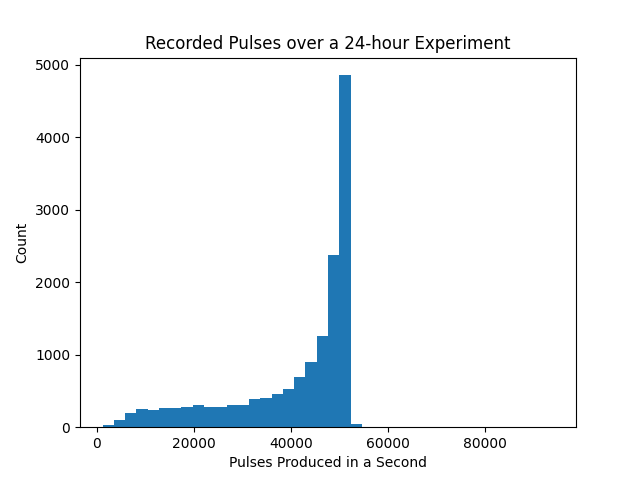
\includegraphics[trim=20 0 50 0,width=3.3in]{figures/sensitivity/loyd10.png}
\caption{The distribution of recorded pulses over time during a pulse count fitness sensitivity experiment}
\label{fig_pulse_sensitvity_1d_hist}
\end{figure}

\begin{figure}[!ht]
\centering
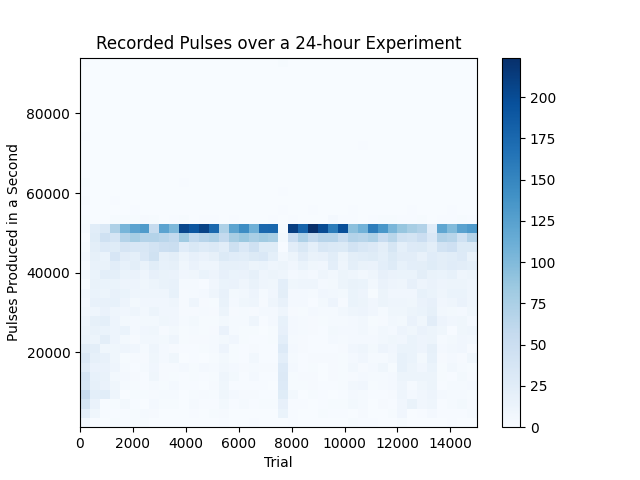
\includegraphics[trim=0 0 50 0,width=3.4in]{figures/sensitivity/loyd11.png}
\caption{The distribution of recorded pulses over time during a pulse count fitness sensitivity experiment}
\label{fig_pulse_sensitvity_2d_hist}
\end{figure}

\begin{figure}[!ht]
\centering
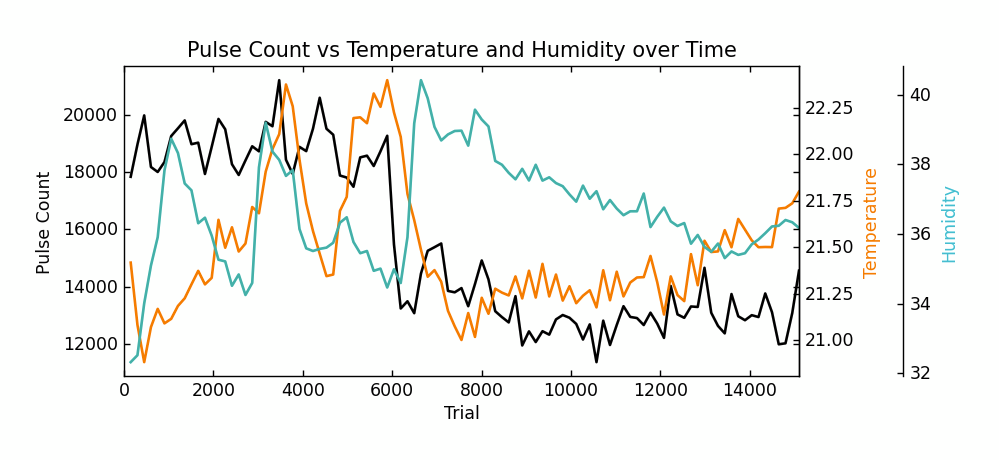
\includegraphics[trim=50 0 50 0,width=3.3in]{figures/sensitivity/loyd12.png}
\caption{The recorded pulse count of a circuit vs the temperature of humidity of the local environment during a fitness sensitivity experiment}
\label{fig_pulse_sensitvity_env_pulse_count}
\end{figure}


\begin{figure}[!ht]
\centering
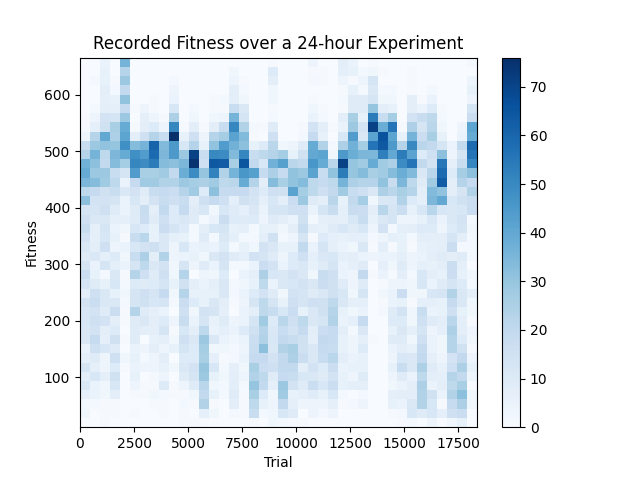
\includegraphics[trim=30 0 70 0,width=3.0in]{figures/sensitivity/loyd13.png}
\caption{The distribution of recorded fitness over 24 hours during a variance maximization fitness sensitivity experiment}
\label{fig_var_sensitvity_2d_hist}
\end{figure}


\subsubsection{Variance Maximization Sensitivity}



To measure the robustness of circuits evolved for variance maximization, we ran a variance maximization experiment (see Appendix \ref{sec_var_max_results}),  recorded the best circuit from every tenth generation, and tested each of these best circuits for three hours without additional changes. We chose to use a shorter sampling duration for these experiments because the fitness distribution stayed relative constant over time. An example of a variance maximization fitness distribution over 24 hours is shown in Figure \ref{fig_var_sensitvity_2d_hist}. These tests were run consecutively to closely match the environment of each experiment. 

We performed a similar analysis to that of the pulse count fitness sensitivity experiments. The correlation between the generation each circuit was pulled from and the standard deviation is 0.19169. The correlation between the generation each circuit was pulled from and the coefficient of variation is 0.004633. 
%Further data from this experiment is shown in section \ref{sec-more-fitness-sensivity}. 
So, for variance maximization experiments, it seems that circuits are neither becoming more nor less stable throughout evolution. Additionally, fitness does not seem to correlate with consistency in behavior.

\section{Discussion} \label{sec_discussion}

% Summary
Our results demonstrate that the \textit{Bitstream Evolution} framework can be used to conduct experiments exploring the evolution and evaluation of circuit behavior.  We have reported on the evolvability of circuits producing different target frequencies, explored the transferability of evolved circuits, and evaluated the robustness of evolved circuits.


% OSC Frequency
Currently, the data suggests it is easier to evolve stable oscillators at certain frequencies.
Generally, a desired frequency 40 kHz seems like a particularly easy target for evolving oscillators. Every frequency tended to see similar progression, making rapid progress initially before plateauing by generation 200. From there, each type of oscillator would continue to make progress, but at a slower rate. The 40 kHz experiments made slower progress after generation 200, while some of the low-fitness oscillators were still making progress (such as the 10 kHz oscillators). The generation best and average fitnesses were sporadic for each type of oscillator. However, the 40 kHz oscillators tended to have a best generation fitness near the other oscillators' best overall fitness. There was similar behavior with the average vs best fitness. More work is needed to determine why a 40 kHz desired frequency tends to produce such stable oscillators.


While experiments in transferability are promising, there is room for improvement. When transferring a circuit from one board to another, we never saw the second board reach the same fitness as the first board right away, always requiring a few generations of evolution. \highlight{From a practical standpoint, this is not feasible since EHD is intended to evolve a final form of a circuit; therefore, a future goal would be to evolve a circuit that could instantly perform on another board with no additional evolution.} The first generation after transfer typically saw greater fitness than randomly-generated circuits would have accomplished, but in all cases, additional evolution on the new board was required to return to similar fitness levels. This evolution would take much less time to reach the fitness of the previous experiment, and in almost all cases was able to produce even better circuits. This suggests that using a previously evolved population of circuits could be used as a better starting population for further experiments, rather than a population of randomly generated circuits. 


% Transfer A - variance max
The variance maximization transferability experiments demonstrated the ability for transferability to escape local minimums and to decrease recovery time. Recovery time (generations to 95\% of the previous interval's final fitness) decreased from 155 generations after the first transfer interval to just 22 generations after the final transfer interval. Ideally, one could evolve circuits with no recovery time and a seamless transition between intervals. While this has not been achieved, the decrease in the recovery time is promising. More work will need to be done to investigate whether properly general circuits can be evolved in this fashion.

% Transfer B - target freq
The target frequency transferability experiment proved more challenging. Although the same pattern of decreased recovery time appeared from the first to the second transition, the third transition actually failed to recover with 200 generations. The population appeared to have converged to a very similar level of average fitness on \textit{FPGA B} as it had originally done on \textit{FPGA A} in the first 100 generations of evolution. Thus, it seems plausible that the components evolved in generation 200-399 on \textit{FPGA B} aided the evolution in generations 400-599 on \textit{FPGA A}. However, with the selection for characteristics of \textit{FPGA A} or just genetic drift, it seems that the beneficial components for  \textit{FPGA B} may have been lost during generations 400-599. More thorough recording of populations and subsequent experimentation and analysis could help verify or refute these ideas. These results parallel Thompson's ``evolvatron" \cite{Thompson1998OnEvolution} both in the cyclic nature of evolution and circuit behavior, but also the challenge of producing a single circuit that operates well on multiple FPGAs.


%Sensitivity analysis introduction
Evolving on a single board in a single environment does not produce immediately transferable results (which is expected), so future work in evolving robust circuits may necessitate new methods to generate transferable circuits (discussed in section \ref{sec_future_work}). However, as another step in making progress towards robust circuits, our experiments on measuring fitness sensitivity, or circuit self-consistency, have helped to illuminate the landscape of reliability for several example behaviors.


%Sensitivity analysis A - Variance Max
For sensitivity in variance maximization experiments, we have pulled circuits from various stages in evolution (different generations). While fitness improves over time (as expected), with the aforementioned correlation between the generation and coefficient of variation being 0.004633, fitness was equally stable for all circuits regardless of the generation the circuit was pulled from. Without specifically basing fitness on consistent behavior, evolution tends to find consistent circuits. It is likely just easier to evolve a consistently noisy circuit than an inconsistently noisy one. Because the time circuits are evaluated for is so short and randomness in timing (upload time, serial communication, CPU task scheduling, etc), the time a particular circuit gets evaluated is effectively random. We believe this is why circuits are equally stable no matter which generation they appear -- an inconsistently noisy circuit would have a low chance of their period of ``noisiness" coinciding with the measurement window. This bodes well for other applications, as we believe this property would extend to other types of fitness evaluation.


%Sensitivity analysis B -Target freq
In the pulse count fitness sensitivity experiments, we examined the impact of target frequency and environmental factors on consistency. We found little to no correlation between target frequency and consistency, measured by the correlation between the mean frequency recorded and the coefficient of variation (which has a value of 0.02394). Additionally, when environmental factors are stable, pulse counts remain relatively stable as well. Significant changes in pulse counts coincided with significant changes in the environment's temperature or humidity, as we will discuss further below. Unfortunately, this means oscillators evolved in this fashion tend to fail in different environments, meaning in the future, further environmental pressure to evolve for robustness must be applied.

%Sensitivity analysis C  std/cov. analysis and implications
In the fitness sensitivity experiments, circuits showed relatively consistent fitness levels over time. Although the fitness functions used are stochastic, there was often not a significant variation in fitness for the same circuit. However, slight variations were present. Currently, we have minimal consideration made in the \textit{Bitstream Evolution} tool to account for this stochastic nature. We do use high elitism in our selection methods and take multiple samples of each circuit every generation. With even these small considerations it seems possible to make consistent progress. 

For the most part, a circuit's fitness seems to stay relatively consistent over time, but some environmental factors besides time, such as temperature and humidity, play a role in the behavior of evolved circuits. Beyond even temperature and humidity, we have evidence of at least one experiment (Figure   \ref{fig_pulse_sensitvity_env_pulse_count}) in which a single circuit evaluated over 24 hours had a drop in fitness corresponding to a sudden change in temperature and humidity. Interestingly, it never returned to the same fitness level again, even after the temperature and humidity returned to the previous measures. Thus, more work is needed to determine what other factors impact circuit behavior. Additionally, the fitness sensitivity of circuits seems to be independent of their average fitness, suggesting at present, evolution neither encourages nor discourages stability.% Ideas for evolving stable circuits will be explored in future work.




%adjust fitness function
%Our efforts to improve the fitness function for the target frequency task as described in this paper are a step in improving the techniques for effectively evolving circuits for various tasks and characteristics. While the $+1$ fitness bonus does assist in preventing timeouts/no-pulse circuits from being rated higher than very high-frequency circuits, it does present other problems. We have observed that using fitness-proportionate selection with the $+1$ fitness can slow evolution in other circumstances. For example, one circuit can have a fitness of 1.02 and another can have a fitness of 1.04. Without the $+1$ bonus, the second circuit would have double the fitness of the first and therefore double the chance of reproducing. With the $+1$ bonus, this circuit now has just an approximately 2\% higher chance to be selected. The remedy is to simply set fitness to zero for no-pulse and timeout instances, and remove the $+1$ bonus entirely. While our current results were gathered using the $+1$ bonus, we will be removing it in the future. 

\section{Future Work} \label{sec_future_work}

The FPGA-intrinsic analog domain of the field of evolvable hardware is still ripe for further development. In this section, we provide our vision for some short and long-term goals for the field. We start with goals to expand the \textit{Bitstream Evolution} toolkit and then discuss some of the theoretical and empirical work that needs to be done to re-establish the field more rigorously. Finally, we outline several fields that we see this work having an impact on and articulate how that may happen in the future.

% toolkit goals
Most immediately, we plan to enhance this toolkit through the development and implementation of an open-source carrier board. This carrier board will support using a Raspberry Pi as the CPU, which will run the \textit{Bitstream Evolution} software. The carrier board will support headers for easy connections to one or more FPGA development boards. The board will also be designed to allow modifying the PID of the USB adapter on the development boards. This will greatly simplify addressing the FPGA boards individually, enabling future experiments exploring transferability and evolution on multiple FPGAs simultaneously. Documentation for this ongoing work can be found on the \textit{Bitstream Evolution} \href{https://github.com/evolvablehardware/BitstreamEvolutionHardware}{hardware repository}. %TODO Insert Link

With this new approach utilizing the carrier board, we plan to allow direct connections to the Raspberry Pi to transmit measurement data. The integration of functionality with the Raspberry Pi itself streamlines the design by eliminating the need for the Arduino Nano, which simplifies the overall setup and facilitates future scalability. Furthermore, this platform enables expandability for gathering additional measurements such as environmental temperature and humidity. The carrier board also features accessible headers for system inputs, which allows for complex experiments and easier external verification through oscilloscopes of the resulting circuit. We hope that this will aid in our ongoing efforts to reproduce the results of Thompson's tone discriminator, similar to that done by \cite{Hoffmann2022CoBEA}.



 



% empirical questions
There are some broader empirical questions we likewise see on the near horizon for this field. We seek to understand the ``ease" of evolving oscillatory circuits with an approximately 40 kHz frequency. Is there a specific source of noise we can identify that allows this? A related but different question we are exploring is, how easily can one evolve a circuit that can function as a radio? Along this line of inquiry, one could ask what are the limitations and opportunities that such circuits could introduce? There are also still broader questions about the potential and limitations of robustness and transferability of evolved circuits. Many possible methods for defining fitness functions and population operators to enhance robustness and transferability are ready to be explored out-of-the-box with \textit{Bitstream Evolution}. We are eager to see what we can discover as we explore ourselves or perhaps learn from others in the community. For instance, systematic exploration of the impact of passes and samples could offer insights into the effectiveness of selection pressure on self-consistency. 

%transferability and evolvatron
As mentioned in the related work (\ref{sec_related_work}), Thompson's work on the ``evolvatron" seemed to indicate challenges for getting a single circuit to work on multiple FPGAs, but this was an early, preliminary work. With a renewed interest in the field, more work can be done to either overcome the challenges or provide insight into the nature of the limitations for circuit robustness and transferability. 
%We also suggest that focusing on evolving a population of circuits with enough quality diversity to either have an immediately high-performing circuit on new hardware, or to have enough genetic material to quickly evolve to find a high performing circuit.
Relating to this are the opportunities afforded by the field of quality diversity \cite{Pugh2016QualityComputation}, which had not yet been formed at the inception of evolvable hardware. There is an opportunity to explore the evolution of high-performing, but behaviorally-diverse, populations of circuits. %For instance, what are the limitations and potential of evolving circuits operating in a certain voltage range? We have begun an exploration of this for the variance maximization task. Similarly, can a quality diversity algorithm with selection pressure for self-consistency enable the evolution of a collection of diversely-behaving, but highly-robust circuits? We have plans to develop a fitness function to explore precisely this for our target frequency task. 
We hypothesize that the diversity and quality of solutions produced should increase the odds of providing better transfer across different physical devices. However, even if circuits do not immediately transfer high-quality behavior, we believe that having a larger pool of diverse solutions greatly increases the odds for evolution to find a ``foothold" to be used to initialize a new population to be evolved on new hardware.



% theoretical questions - intermediate representations
While the work done to date has been performed at the level of bitstream manipulations (i.e. pseudorandom bit flips), there is an opportunity to devise intermediate representations, either through direct or indirect encodings of the genome for defining circuits. Incorporating these into the \textit{Bitstream Evolution} is a promising direction, and our work may build on prior work in this area \cite{Shanthi2009PracticalCircuits,Torresen2002AHardware,Gordon2005}. Although evolution has found ways to take advantage of disconnected components that still serve a functional purpose in evolved circuits, it would be interesting nonetheless, to aim for explicit mutations resulting in additions or deletions of connected components. Taking such an approach has the potential to both rapidly increase the rate of evolution and result in less time exploring circuits that might not have any functional impact on existing circuits. It also might result in the evolution of circuits that are more reliable or transferable given a more strict set of constraints. Although not yet reported, preliminary efforts to investigate the minimal number of logic blocks required to evolve circuits for some of the basic circuit behaviors reported in this paper are currently underway. Such efforts focus on generating the minimally sufficient qualitative behavior of an output waveform by constraining the number of resources available throughout the evolutionary process, such as an analog pulse oscillator evolved with fewer than 25 CLBs or targeting the maximum signal variance for a circuit with 10 CLBs. Further investigation of these resource deprived circuits, as well as exploration of evolution using high-order representations of circuit genomes, is likely to reveal the deeper potential and challenges in the field.


% fields to have application
As progress is made in these different areas it may open up new avenues in other fields. One area of work is in computer security. If it were possible to manipulate bits or read signals in disconnected components, it would open a wide range of possible exploits. For signal processing on embedded devices such as satellites, the need for efficiency is paramount, and often there may be limitations for power and physical space. For such conditions, evolvable hardware stands to push the bounds of what is feasible with creative uses of electronic components. Additionally, usage of these algorithms allows for circuits to be fine-tuned for specific Digital Signal Processing (DSP) applications or use cases. These specialized circuits can have performance benefits over the general-purpose tools and algorithms commonly used in DSP applications, in terms of performance, power usage, efficiency, physical space, etc.


Beyond these areas, with the ongoing AI revolution, the need for more efficient and neuromorphic approaches to hardware is as promising as ever. The long-standing von Neumann architecture is facing increasing strain, and increasingly specialized or reconfigurable hardware is being developed and deployed. The intrinsic analog evolvable hardware research we seek to advance with this toolkit is being applied to an FPGA designed for digital computation, but can help to answer questions about the opportunities and limitations of evolvable hardware more broadly. For instance, recent work in hardware accelerated neuroevolution \cite{Whitley2024NeuroevolvingNetworks} has shown that utilizing reconfigurable hardware such as multi-processor system on chip (MPSoC) based FPGAs and methods of intrinsic evolution drastically increases circuit evaluation and the rate of evolution for Continuous-Time Recurrent Neural Network models. Such time-integral, dynamic neural models are becoming increasingly important for computationally constrained edge-devices that perform signal-processing tasks such as sensor fusion and embodied, closed-loop systems that are often subject to out-of-distribution inputs that must be handled gracefully. When evolution has the opportunity to tap into signals, timescales, and continuous values that are inaccessible to modern digital computing, we can expect challenges, but also tremendous opportunities. We hope that this paper and the associated toolkit will help push forward this field.

\section{Conclusion}
In this paper, we presented the \textit{Bitstream Evolution} platform, which aims to advance research in the domain of intrinsic, bitstream-level, evolvable hardware. The platform is designed to facilitate community engagement and contributions by providing open-source software,  accessible tutorials, and a publicly available result repository. We strive to enable iterative enhancements by researchers globally to address the challenges and open questions in the field. 




Using this platform we reported on findings from several experiments focused on the robustness and transferability of circuits evolved on modern hardware. These results show promising outcomes in the robustness and transferability of evolved circuits. %The results also suggest several important lines of inquiry, such as identifying possible sources of noise that evolution repeatedly identifies in the 40 kHz range when evolving oscillatory circuits.
Anyone can easily and productively contribute to this open domain of science through 1) re-running these same experiments with their personal hardware to help verify the reproducibility across a wider range of environments and 2) re-running these experiments with a different range of parameters. We provide tutorials on running first-time experiments in the appendix (\ref{sec_walkthrough}). However, this paper reports on a wider range of experimental setups, but all are capable of running out of the box.

Looking ahead, the platform sets the stage for exploring numerous avenues within evolvable hardware. Open questions about stability, transferability, robustness, and quality diversity remain, presenting exciting opportunities for further research. Our discussion of future directions includes enhancing the platform's capabilities to support more diverse experimental setups, which could significantly impact the adaptability and applicability of evolved circuits across different hardware configurations and operational conditions. 

The collaborative and open-source nature of the \textit{Bitstream Evolution} platform is designed to accelerate the pace of innovation in this field. By lowering the barriers to entry and encouraging global participation, we aim to foster a vibrant community of researchers dedicated to pushing the boundaries of what's possible with evolvable hardware.

\begin{appendices}
\section{\break Example Experiment Tutorials} \label{sec_walkthrough}
This section walks through two sample experiments to illustrate how to use the system, along with the results from running these experiments. The goal of each experiment is to reproduce prior results quickly. In this section, we will walk through the key configuration parameters and explain how these will affect each experiment. Each experiment will contain a table of relevant configuration parameters (parameters that are excluded are irrelevant for the particular mode; must be configured per system, such as file paths, or are not the subject of the experiment and should be left at default values, such as the routing type). Additionally, each section will include plots generated from running the experiment to give an idea of what results should look like.




\clearpage
\newpage


\subsection{Variance Maximization Experiment}
\label{sec_var_max_results}
This first experiment uses the variance-maximization fitness function to evolve circuits that generate noisy signals, which is the easiest type of experiment for which to get rapid, positive results. The full list of relevant configuration settings is in Table \ref{example_config_table}. Additionally, the configuration file for the experiment outlined here is present in the \textit{Bitstream Evolution} \href{https://github.com/evolvablehardware/BitstreamEvolution/blob/main/data/example_configs/variance_maximization.ini}{GitHub repository}. 

%\jason{make hyperlink to repo here}
%In general, users can expect to see positive results within 200 generations, though the capacity of these results may vary depending on the environment. 

Next, we will provide explanations for the parameter values chosen and how those parameters operate, when not immediately clear. Whether or not to perform a mutation is evaluated on a per-bit basis, so a low mutation rate can still lead to many mutations in a single individual (with a bitstream of 1728 bits, this rate of 0.0021 results in an average of 3.6 bits flipped per individual each time that individual is mutated). Due to the nature of the stochastic fitness function (particularly when evolving intrinsically), high elitism is important, as a single broken connection can send a once-good circuit to a fitness of zero. Fitness-proportionate selection (FIT\_PROP\_SEL) is used, because it heavily favors high-fitness elites.
%, and the fitness of a circuit scales linearly with its ``performance". 
We use the random initialization mode to evolve circuits completely from scratch.

Running this experiment ought to produce results similar to those in Figure  \ref{canonical_varmax}. Note that these plots were generated by running the experiment for 500 generations rather than 200; however, all other parameters were the same. We primarily analyze the performance of the best circuit, which, as we can see, made jumps at around 100 and 200 generations before not making any additional improvements throughout the experiment. Diversity, as expected, drops significantly after the completely randomized population settles on a particular genotype.

In Figure \ref{canon_waveform}, we can see the waveform generated by the highest-fitness individual in the final generation. As expected, it is fairly noisy, frequently leaping between the low and high voltage levels. The trigger voltage line refers to the threshold between what is considered a logic low and a logic high on the microcontroller. As we can see here, this circuit frequently crosses this threshold, and we would expect it to produce a large number of pulses using the pulse count fitness function.%, which counts the number of times the signal crosses from low to high.



%\begin{figure}[!ht]
%\centering
%\includegraphics[width=3.5in]{figures/plot_samples/canon_violin.png}
%\caption{Violin plots from variance-maximization experiment}
%\label{varmax_violin}
%\end{figure}

%\WIP{
%Figure \ref{varmax_violin} shows violin plots for the population fitnesses every 50 generations. Populations tend exhibit an hourglass shape, with several high-fitness individuals and a large cluster of lower-fitness individuals. We can see that around generation 400, there were not many high-fitness individuals; cross-referencing with figure \ref{canonical_varmax}, we can see the average fitness dipped at generation 400.
%}



The final plot that this experiment will generate is the voltage heatmap, shown in Figure \ref{varmax_heatmap}. This plot shows the frequency of voltage levels for the best circuit in each generation. For example, for approximately the first 100 generations, readings of the voltage of the best circuit were between 0 and 0.5 volts, but typically somewhere in between. In later generations, it was more common to get readings at either 0 or 3.3 volts. The population made its first big jump around generation 100, which is consistent with the findings here.

\begin{table}[!h]
\caption{Table of Relevant Configuration Parameters
\label{example_config_table}}
\centering
\begin{tabular}{|c|c|}
\hline
Parameter & Value \\
\hline
\tt{population\_size} & \tt{50} \\
\hline
\tt{generations} & \tt{200}\\
\hline
\tt{target\_fitness} & \tt{IGNORE} \\
\hline
\tt{fitness\_func} & \tt{VARIANCE} \\
\hline
\tt{mutation\_probability} & \tt{0.0021} \\
\hline
\tt{crossover\_probability} & \tt{0.7} \\
\hline
\tt{elitism\_fraction} & \tt{0.1} \\
\hline
\tt{selection} & \tt{FIT\_PROP\_SEL} \\
\hline
\tt{randomize\_until} & \tt{NO} \\
\hline
\tt{init\_mode} & \tt{RANDOM} \\
\hline
\tt{simulation\_mode} & \tt{FULLY\_INTRINSIC} \\
\hline
\end{tabular}
\end{table}



\begin{figure}[!h]
\centering
\includegraphics[width=0.475\textwidth]{figures/plot_samples/loyd14.PNG}
\caption{Fitness values and diversity for one run of the variance-maximization example experiment.}
\label{canonical_varmax}
\end{figure}


\begin{figure}[!h]
\centering
\includegraphics[width=0.45\textwidth]{figures/plot_samples/loyd15.PNG}
\caption{Waveform of best circuit in the variance-maximization experiment.}
\label{canon_waveform}
\end{figure}



\begin{figure}[!h]
\centering
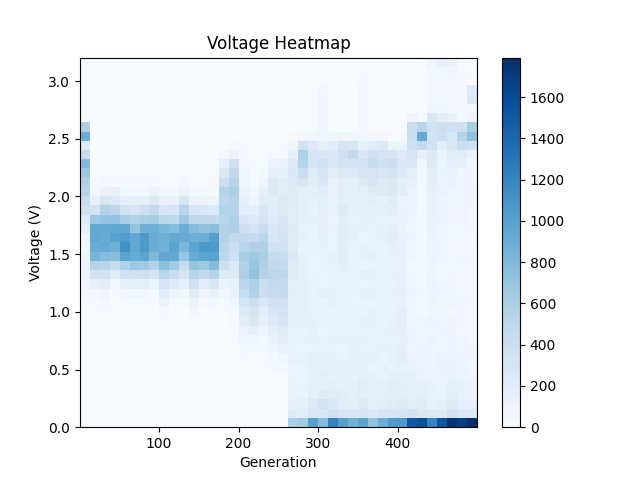
\includegraphics[width=0.5\textwidth]{figures/plot_samples/loyd16.png}
\caption{Heatmap for circuit voltage levels in the variance-maximization. Initially, circuits remain at a low voltage but evolve to alternate between high and low.}
\label{varmax_heatmap}
\end{figure}


\clearpage
\newpage

\subsection{Pulse Count Oscillator Experiment}
\label{sec_pulse_count_results}


This next experiment uses the pulse count fitness function to evolve oscillator circuits. Again, the full list of relevant configuration settings is provided in Table \ref{sample_pulse_config_table}, and the configuration file for the experiment outlined here is present in the \textit{Bitstream Evolution} \href{https://github.com/evolvablehardware/BitstreamEvolution/blob/main/data/example_configs/40k_oscillator.ini}{GitHub repository}.
% \jason{add hyperlink to repo}

We have found positive results in less than 500 generations. However, we have provided plots for this same experiment run for 500 generations and recommend running it for that long to achieve results similar to those in Section \ref{freq_cmp_section}.

Many of the parameters are the same as the variance-maximization experiment for the same reasons. We use the randomization feature to randomize bitstreams until we find a circuit that produces a non-zero number of pulses. Then, the evolutionary process begins; this ensures that you will start with an initial population of pulse-producing circuits for evolution to build off of. We have found that the tolerant and sensitive fitness functions tend to produce similar-caliber oscillators, so, because it has historically been used more often, we will be using the sensitive function. Additionally, because 40 kHz oscillators tend to be the most successful, we will set that as our target frequency.

In Figure \ref{canon_pulse_main}, the pulse count experiment at first seems fairly unsuccessful, \highlight{reaching the ideal fitness of 1 twice, but not consistently}. However, it's important to note that this fitness function is fairly unforgiving. \highlight{The jumps in best fitness up to values of 0.5 or 0.25 represent getting within 1 and 2 pulses of the target respectively, which is extremely difficult with such a high target fitness (being just 10 pulses off of a target of 40,000 results in a fitness of 0.1).} We'll take a look at the pulse count graph to get more illuminating results.

The plot in Figure \ref{canon_pulse_pulses} displays data for the pulses counted, rather than the fitnesses. A red dashed line is drawn for the target frequency for reference. There are lines for the ``best" pulse count for that generation (this is the count that is closest to the target), one each for the maximum and minimum pulses counted, and for the population average pulse count. 

%the pulse count experiment was able to relatively quickly evolve an individual with a near maximal fitness score. Additionally the population average fitness and worst fitness did not experience too large of a change for most of the experiment. Diversity starts by steadily increasing, as expected (since we initialize our population from a single seed circuit). Although it seems to fluctuate frequently, this is on a smaller scale (\jason{add in specific numbers 800 vs 100 etc}) than the first sample experiment, where initial diversity was extremely high due to a random population.

For this experiment, the maximum inconsistently oscillated between being very large or being near the target\highlight{, though eventually settled down very close to the target fitness. The minimum did not fluctuate much at all, staying at 0, indicating that there was never a generation without a 0-pulse individual}. There tends to be a higher frequency of low pulse counts versus high pulse counts (as seen below in Figure \ref{canon_pulse_heatmap}), which means the population average tends to be pulled below the target. Here, we can better analyze the performance of the best circuit than with raw fitness, and see that it clearly gets very close to the target frequency \highlight{almost immediately} and stays there for the remainder of the experiment.

Figure \ref{canon_pulse_heatmap} shows the heatmap for pulse counts for each generation of the example oscillator experiment. \highlight{We can see that the population tended to hover both around the target of 40,000 pulses and around 0 pulses. This indicates that many of the mutations simply stopped pulses from being generated at all, rather than slightly changing the number -- demonstrating a key challenge of evolvable hardware.}


\begin{table}[!h]
\caption{Table of Relevant Configuration Parameters
\label{sample_pulse_config_table}}
\centering
\begin{tabular}{|c|c|}
\hline
Parameter & Value \\
\hline
\tt{population\_size} & \tt{50} \\
\hline
\tt{generations} & \tt{500}\\
\hline
\tt{target\_fitness} & \tt{IGNORE} \\
\hline
\tt{fitness\_func} & \tt{SENSITIVE\_PULSE\_COUNT} \\
\hline
\tt{desired\_freq} & \tt{40000} \\
\hline
\tt{mutation\_probability} & \tt{0.0021} \\
\hline
\tt{crossover\_probability} & \tt{0.7} \\
\hline
\tt{num\_samples} & \tt{2} \\
\hline
\tt{num\_passes} & \tt{1} \\
\hline
\tt{elitism\_fraction} & \tt{0.1} \\
\hline
\tt{selection} & \tt{FIT\_PROP\_SEL} \\
\hline
\tt{randomize\_until} & \tt{PULSE} \\
\hline
\tt{randomize\_threshold} & \tt{0} \\
\hline
\tt{init\_mode} & \tt{RANDOM} \\
\hline
\tt{simulation\_mode} & \tt{FULLY\_INTRINSIC} \\
\hline
\end{tabular}
\end{table}


\begin{figure}[!ht]
\centering
\includegraphics[width=0.49\textwidth]{figures/plot_samples/loyd17.png}
\caption{Results of running the pulse count example experiment}
\label{canon_pulse_main}
\end{figure}

\begin{figure}[!ht]
\centering
\includegraphics[width=0.49\textwidth]{figures/plot_samples/loyd18.png}
\caption{Plot of the best, average, and worst pulses counted for each generation}
\label{canon_pulse_pulses}
\end{figure}

\begin{figure}[!ht]
\centering
\includegraphics[width=0.49\textwidth]{figures/plot_samples/loyd19.png}
\caption{Heatmap for pulses counted in the example oscillator experiment}
\label{canon_pulse_heatmap}
\end{figure}


\end{appendices}

\clearpage
\newpage
\section*{Acknowledgment}
% The preferred spelling of the word ``acknowledgment'' in American English is
% without an ``e'' after the ``g.'' Use the singular heading even if you have
% many acknowledgments. Avoid expressions such as ``One of us (S.B.A.) would
% like to thank $\ldots$ .'' Instead, write ``F. A. Author thanks $\ldots$ .'' In most
% cases, sponsor and financial support acknowledgments are placed in the
% unnumbered footnote on the first page, not here.


We would like to express our thanks to Thomas Bioren, Isaac Mierow, Vineet Ranade, Rebecca Testa\highlight{, Kieran Hall, and Brooklyn Jennings} for helping to conduct some of the experiments and ongoing work to improve this toolkit. ChatGPT was utilized to aid in rewording small sections of the paper.



\bibliographystyle{IEEEtran}
\bibliography{mendeley_references}

\vskip -2\baselineskip plus -1fil
\begin{IEEEbiography}[{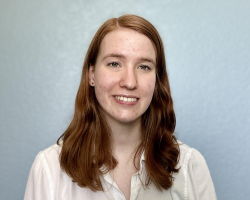
\includegraphics[width=1in,height=1.25in,clip,keepaspectratio]{figures/bios/loyd.png}}]{Allyn Loyd}
is \highlight{currently pursuing a PhD in Industrial Engineering at the University of Houston. They are a recent graduate of Rose-Hulman Institute of Technology, with majors Computer Science and Math. They are also interested in operations research, transportation theory, and robust optimization.}
\end{IEEEbiography}
\vskip -2\baselineskip plus -1fil

\begin{IEEEbiography}[{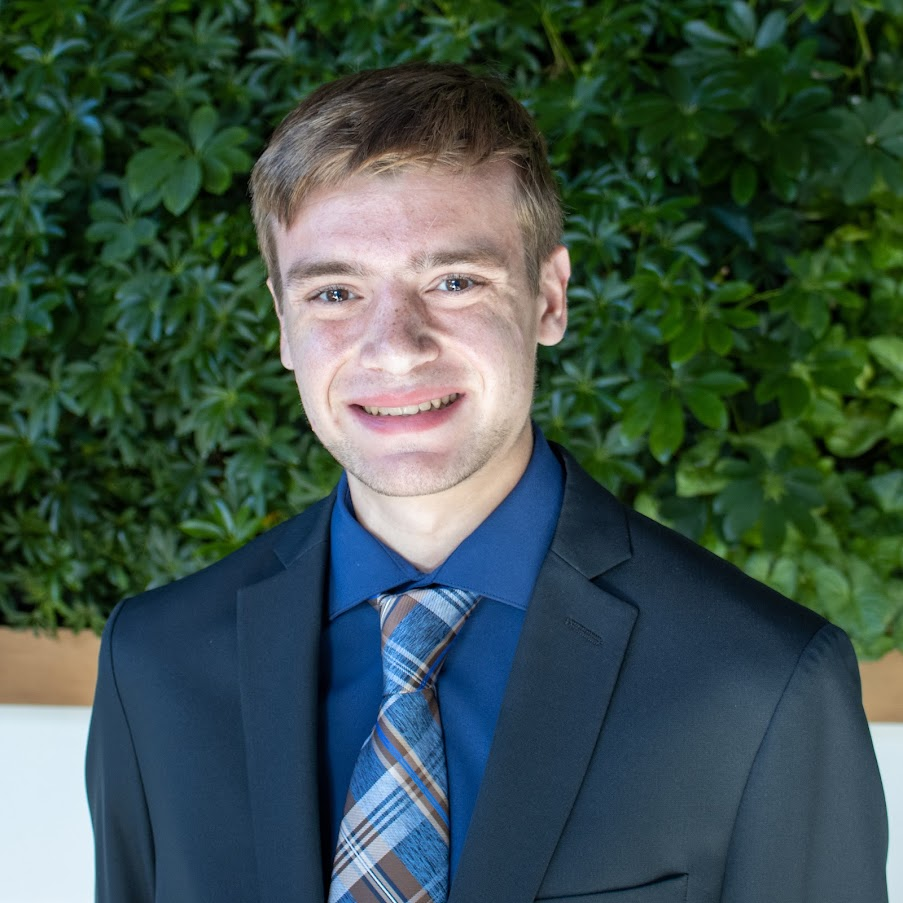
\includegraphics[width=1in,height=1.25in,clip,keepaspectratio]{figures/bios/gaull.jpg}}]{Daniel Gaull}
is \highlight{currently a software engineer at Tesla, Inc. He recently graduated from the Rose-Hulman Institute of Technology with majors} in Computer Science and Software Engineering. He is curious about embedded systems, user-friendly design, and deep learning. 
\end{IEEEbiography}
\vskip -2\baselineskip plus -1fil

\begin{IEEEbiography}[{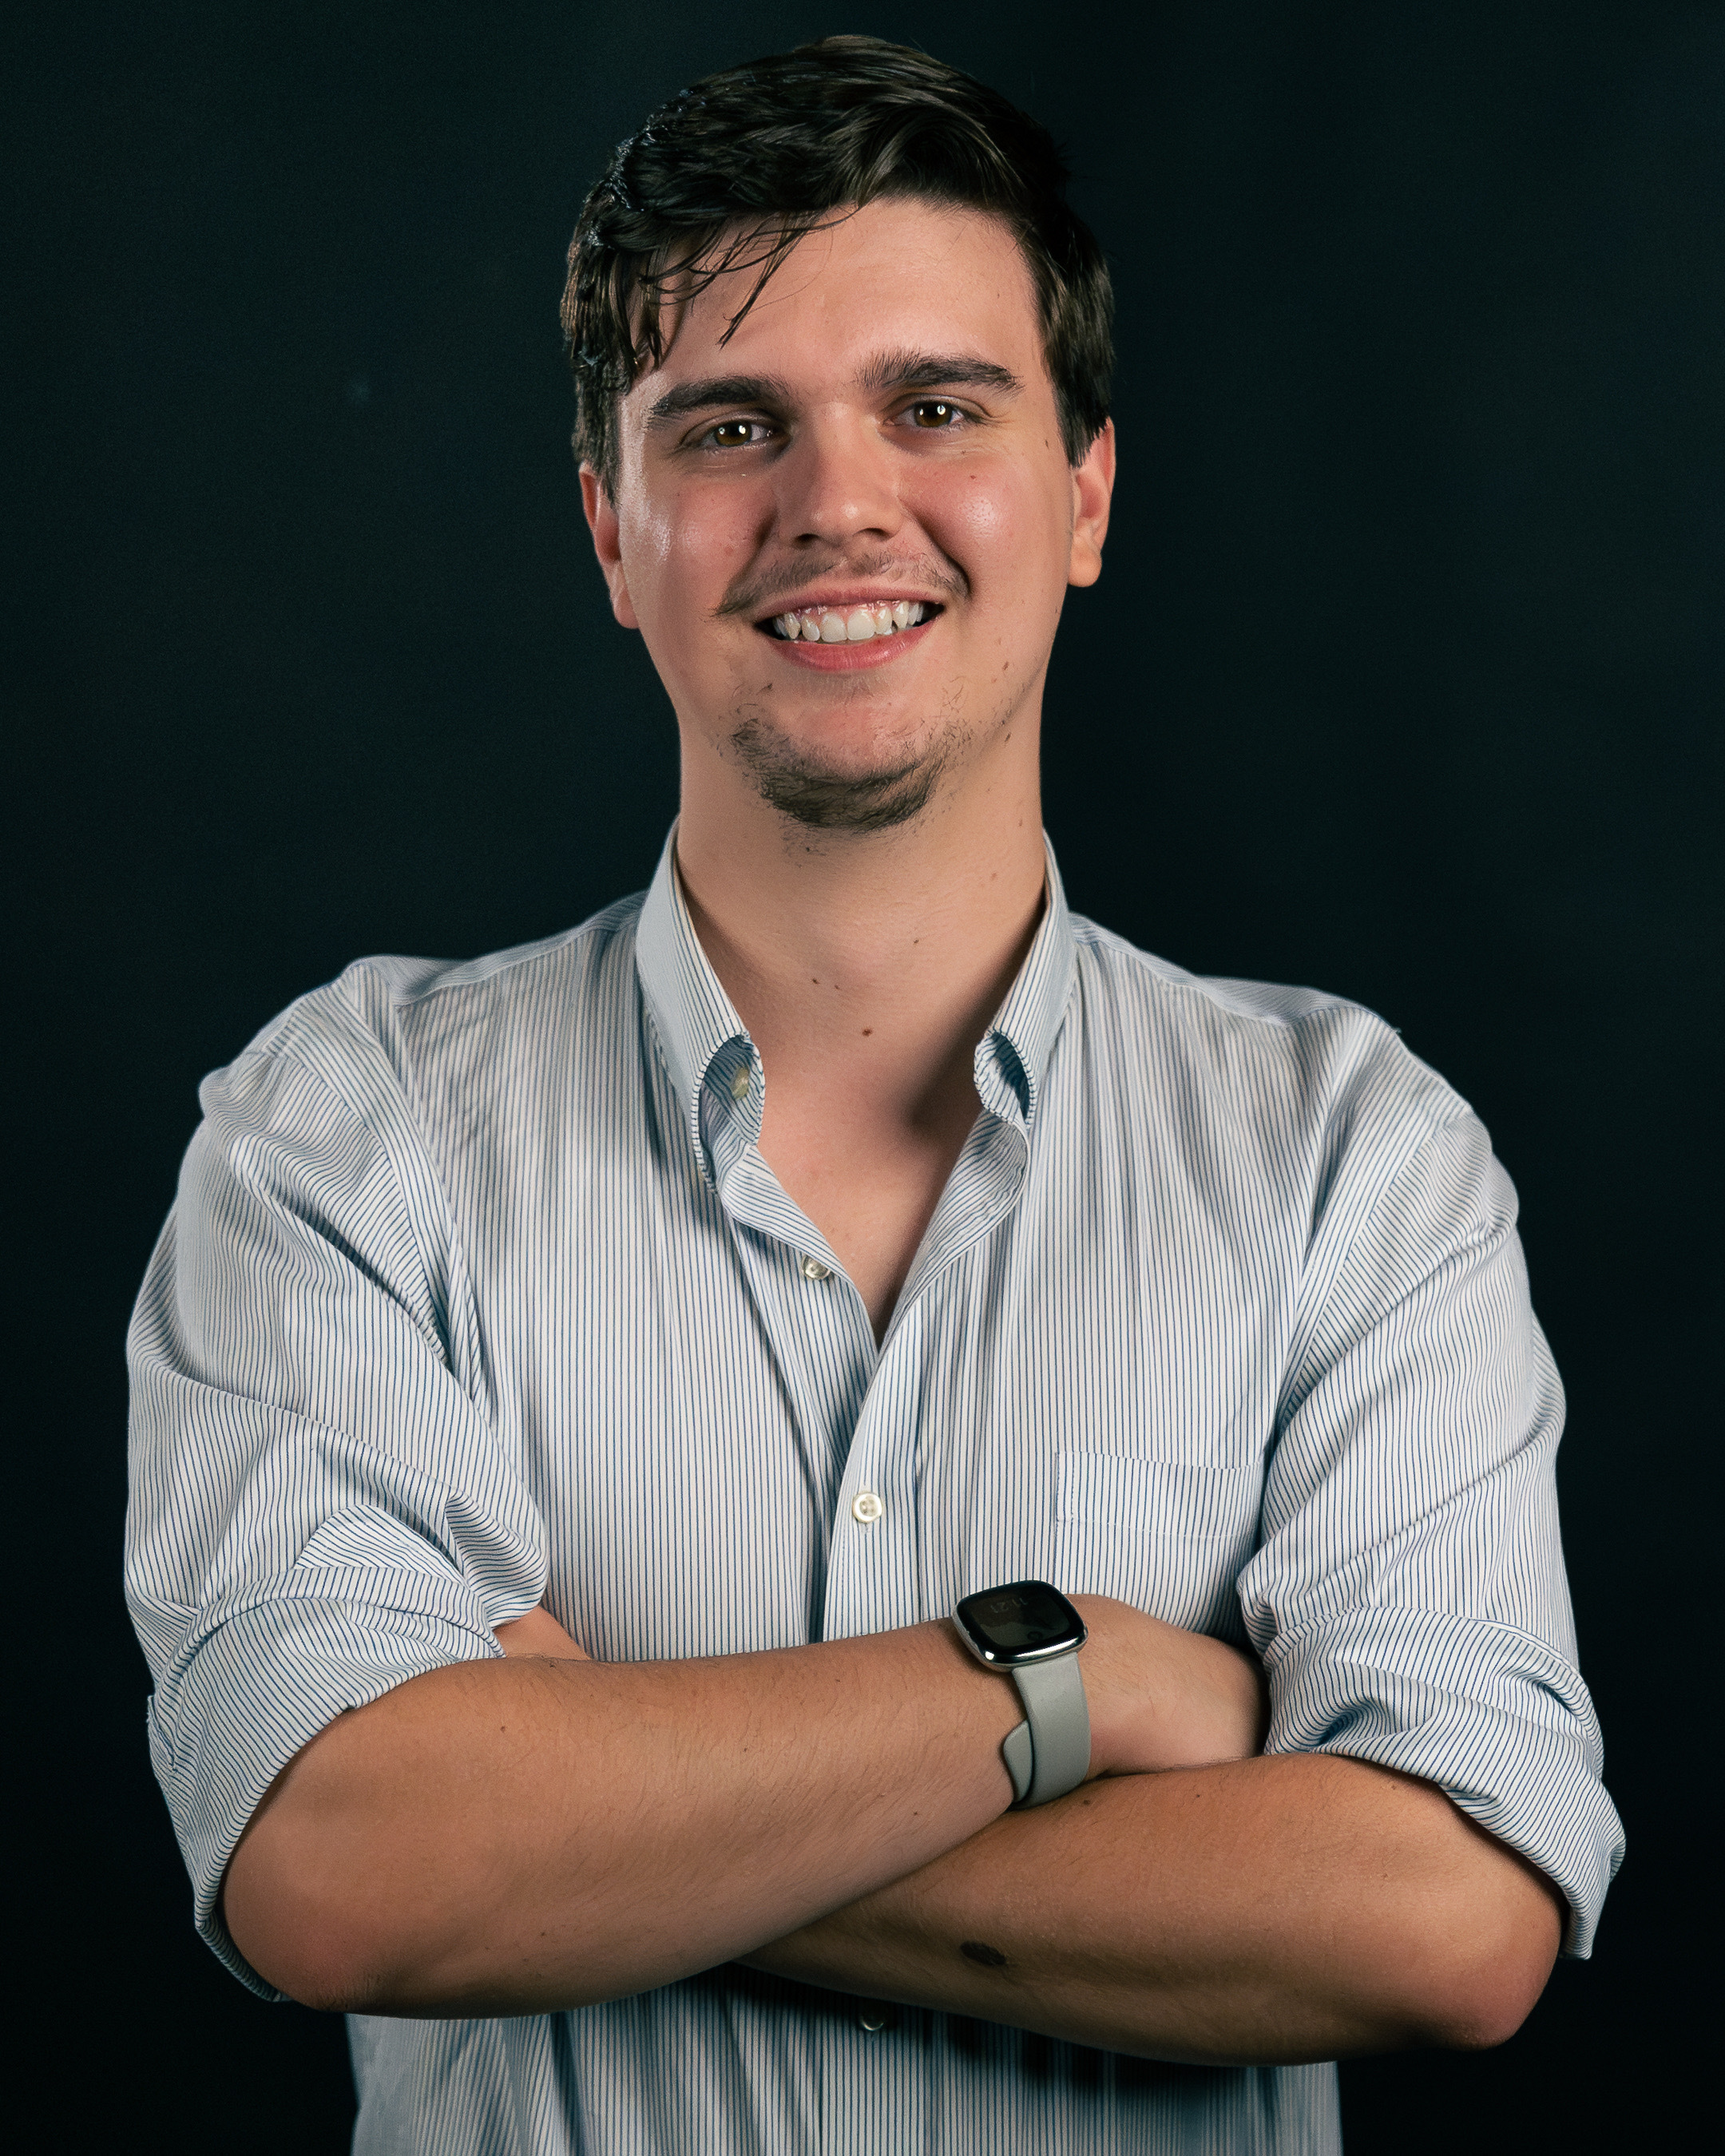
\includegraphics[width=1in,height=1.25in,clip,keepaspectratio]{figures/bios/logan_manthey.JPEG}}]{Logan Manthey}
is currently \highlight{working as a FPGA engineer at Vivum AI. He is a recent gradate of Rose-Hulman Institute of Technology, with a Bachelors of Computer Engineering and Master of Engineering Management. His research interests include embedded systems, hardware acceleration, and neural network implementations on FPGAs.}
\end{IEEEbiography}
\vskip -2\baselineskip plus -1fil

\begin{IEEEbiography}[{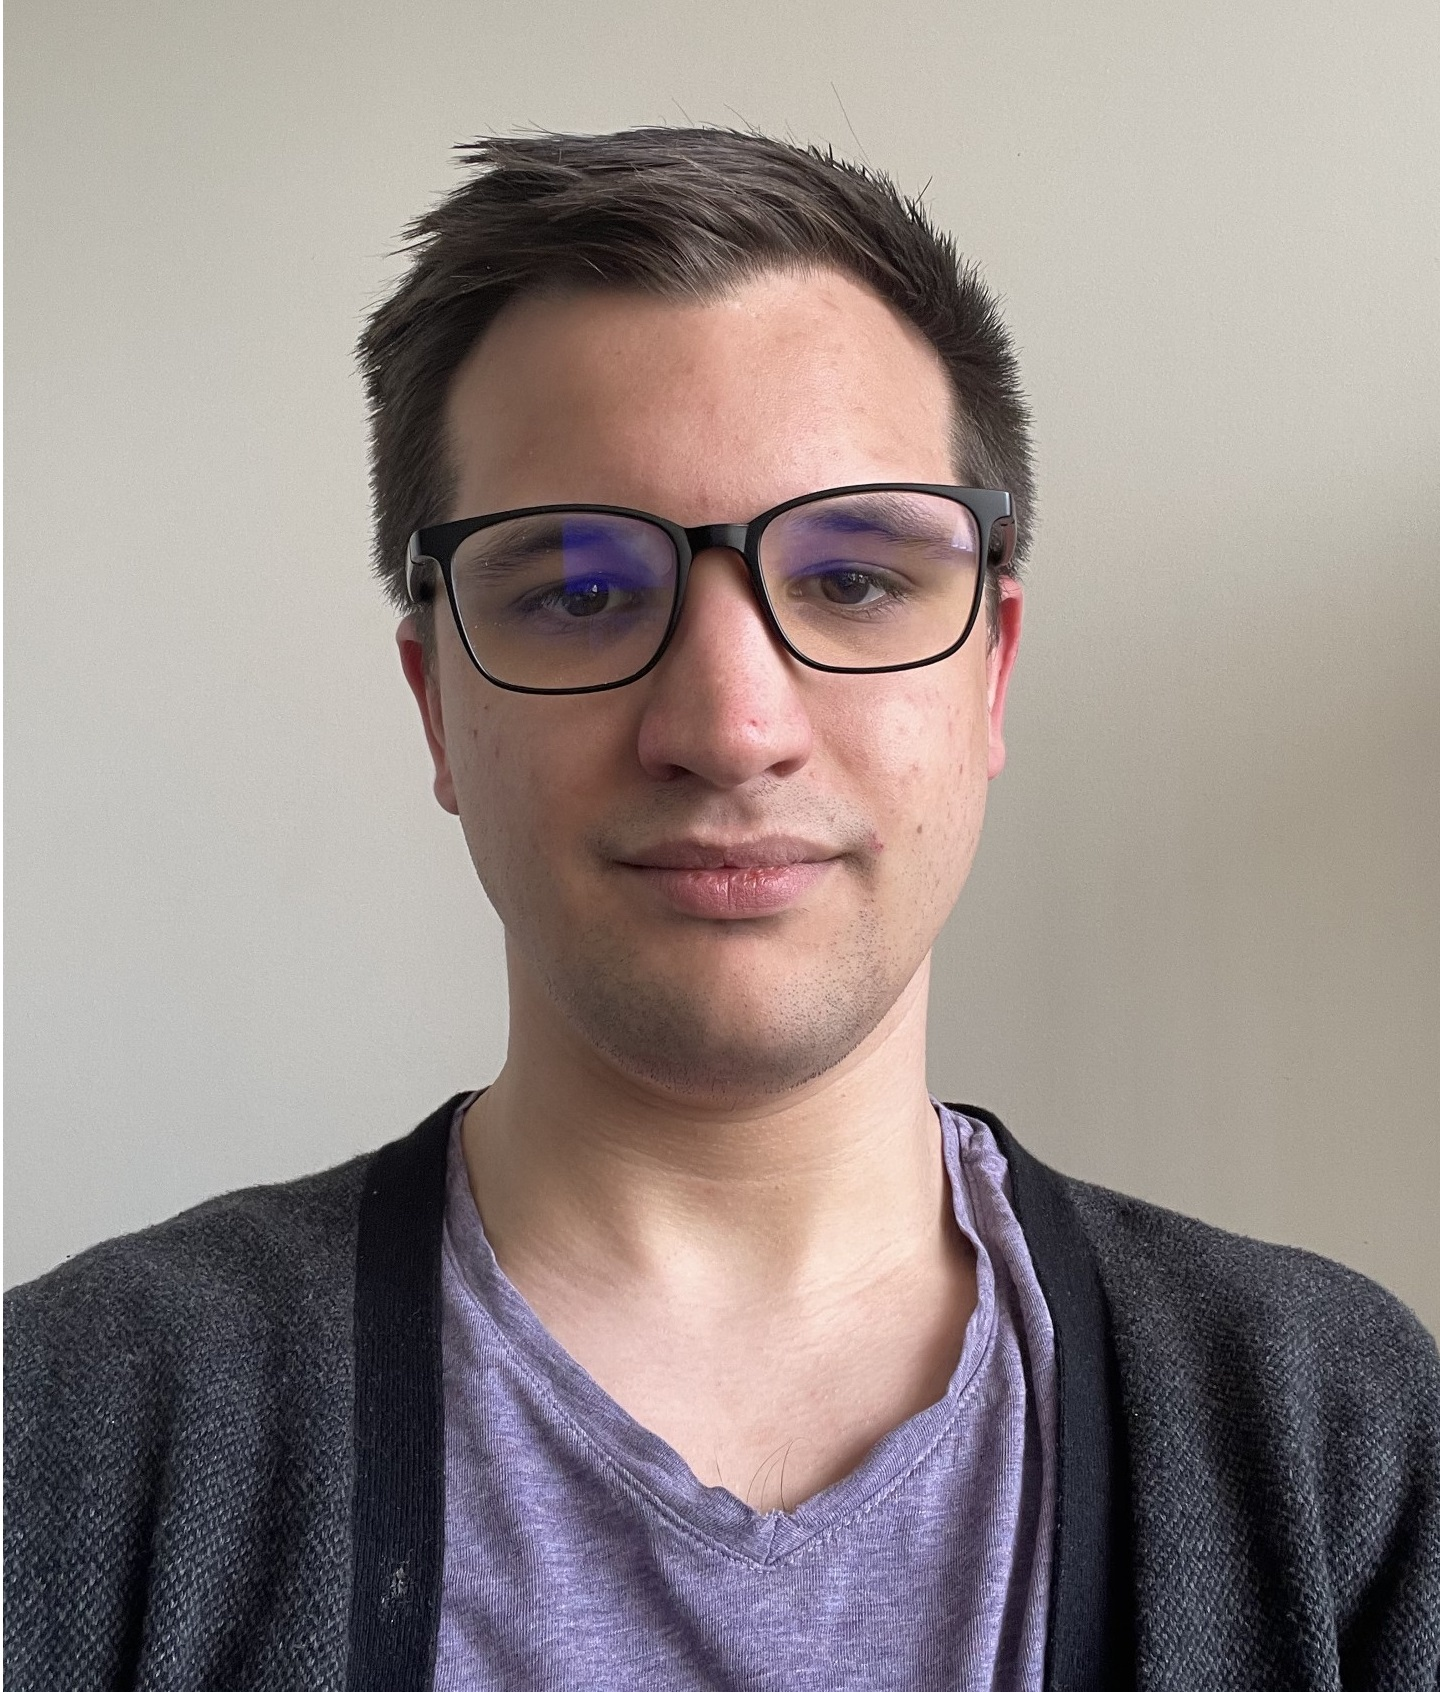
\includegraphics[width=1in,height=1.25in,clip,keepaspectratio]{figures/bios/nicklas.jpg}}]{Nicklas Carpenter} graduated Rose-Hulman Institute of Technology with a Bachelor's of Science in Computer Engineering and a minor in Computer Science. He is currently \highlight{pursuing a PhD in Computer Science at the University of Arizona researching abstract interpretation, program analysis, and computational complexity theory.}
\end{IEEEbiography}
\vskip -2\baselineskip plus -1fil

\begin{IEEEbiography}[{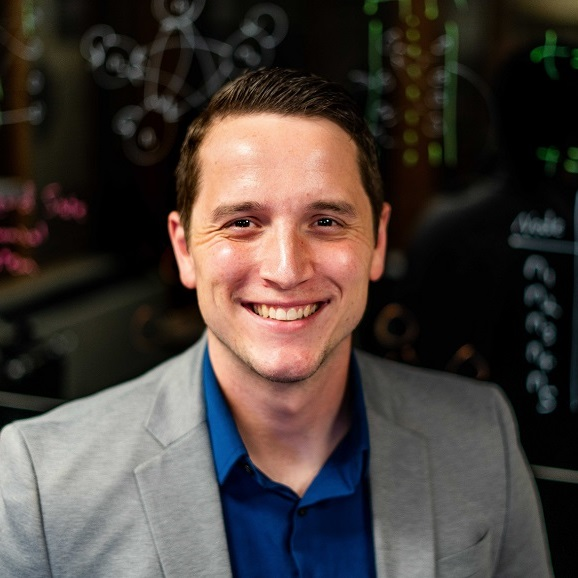
\includegraphics[width=1in,height=1.25in,clip,keepaspectratio]{figures/bios/derek.jpg}}]{Derek Whitley}
holds a dual PhD in complex systems and cognitive science from Indiana University, is the CTO and co-founder of Vivum AI, and is Visiting Assistant Professor at Rose-Hulman Institute of Technology in Computer Science and Software Engineering. His research interests focus on the application of  evolvable hardware, robotics, and neuroethology to both industry and scientific enterprises.
\end{IEEEbiography}
\vskip -2\baselineskip plus -1fil

\begin{IEEEbiography}[{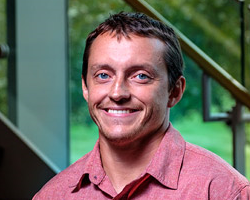
\includegraphics[width=1in,height=1.25in,clip,keepaspectratio]{figures/bios/yoder1_250_200.png}}]{Jason A. Yoder}
earned a dual PhD in computer science and cognitive science from Indiana University in 2018. He is currently an \highlight{Associate} Professor at Rose-Hulman Institute of Technology in Computer Science and Software Engineering.
His research interests focus on evolutionary and adaptive systems that include elements of evolution, development, and/or learning. %Within these fields he has worked on several different research projects individually or with students including developmental artificial neural networks, bio-inspired reinforcement learning rules for continuous-time recurrent neural networks, evolvable hardware, modeling evolutionary development, and various computational models of neuromodulation for artificial neural networks. 
 He enjoys teaching courses such as bio-inspired AI and object-oriented software development. 
\end{IEEEbiography}
\vskip -2\baselineskip plus -1fil

\EOD

\end{document}


% Notes on converting formatting

% When preparing your graphics IEEE suggests that you use of
one of the following Open Type fonts: Times New Roman, Helvetica, Arial, Cambria, and Symbol. 

% Matplotlibs' default font is DejaVu Sans.

% Figures (line artwork or photographs) should be named start-
ing with the first 5 letters of the author’s last name. The
next characters in the filename should be the number that
represents the sequential location of this image in your article.
For example, in author ‘‘Anderson’s’’ paper, the first three
figures would be named ander1.tif, ander2.tif, and ander3.ps.
Tables should contain only the body of the table (not the
caption) and should be named similarly to figures, except that
‘.t’ is inserted in-between the author’s name and the table
number. For example, author Anderson’s first three tables
would be named ander.t1.tif, ander.t2.ps, ander.t3.eps.
Author photographs should be named using the first five
characters of the pictured author’s last name. For example,
four author photographs for a paper may be named: oppen.ps,
moshc.tif, chen.eps, and duran.pdf.
